\documentclass[a4paper,man,natbib,floatsintext,import]{apa6}

\usepackage{longtable}
\usepackage[english]{babel}
\usepackage[table]{xcolor}
\usepackage{lscape}
\usepackage[utf8x]{inputenc}
\usepackage{amsmath}
\usepackage{graphicx}
\usepackage[colorinlistoftodos]{todonotes}
\usepackage{pdfpages}

\title{Analogical Transfer in a Hebb Repetition Paradigm}
\author{Oesch Adrian}
\affiliation{University of Zurich}
\shorttitle{Analogical Transfer in a Hebb Repetition Paradigm}
\begin{document}

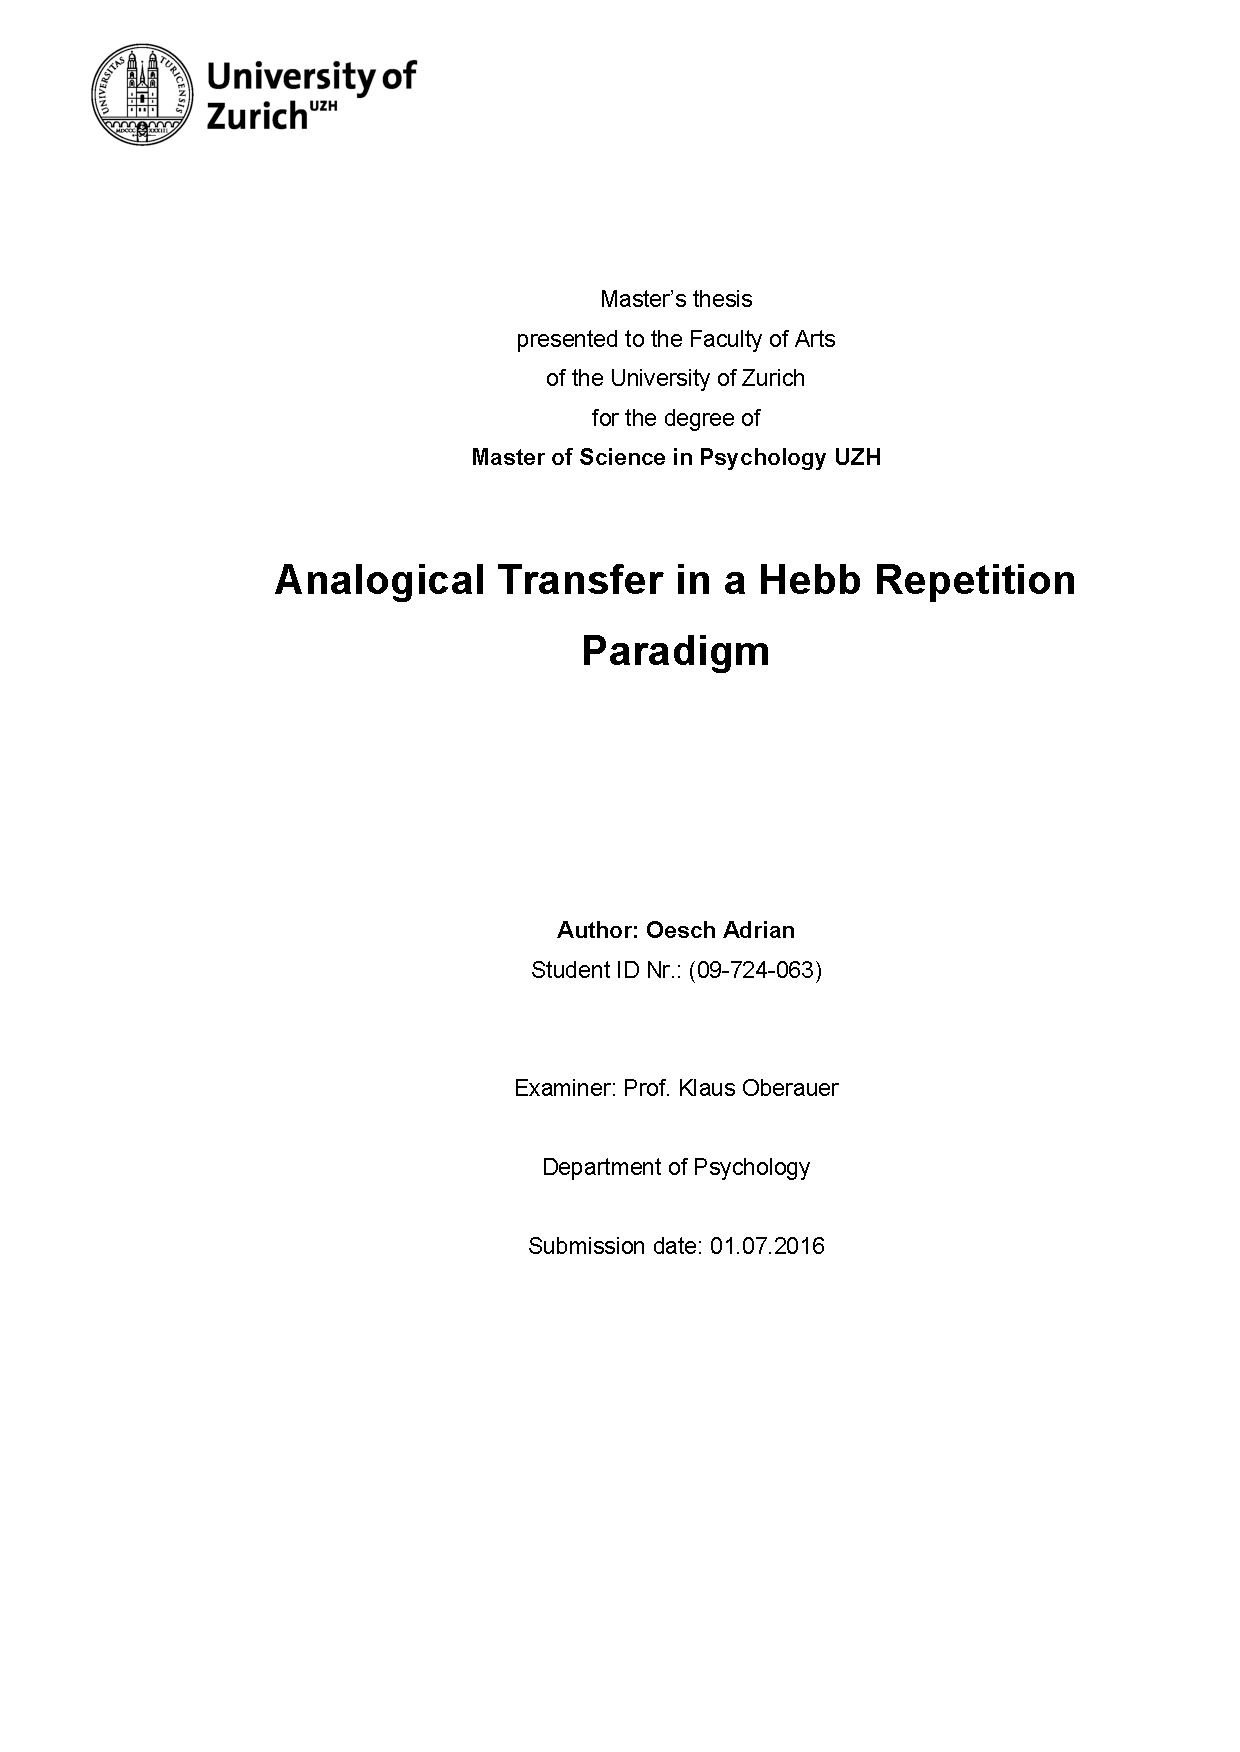
\includepdf{cover}
\section*{Abstract}
Previous research has shown unintentional analogical mapping processes due to relational similarity when participants process word pairs \citep{Popov2015,Estes2006}. Also, it has been shown that structural similarity guides analogical retrieval in reminding studies \citep{Wharton1996}. This thesis aims to combine those lines of research and investigates unintentional analogical transfer on the basis of mere structural similarity. By combining an established method from memory research with original story material, we developed a novel experimental setting to investigate this hypothesis and contribute to growing evidence that analogical transfer is not a deliberative reasoning process but happens also unintentionally. We detected weak evidence (5\%-sign. level) for this effect in experiment 1, where we observed an increased recall performance over trial index in stories with high structural similarity compared to stories with low structural similarity. This effect could not be replicated in experiment 2, where we changed the trial sequence to a repeated condition setting and introduced limited reading time. We then discuss the differences of those two experiments, further methodological improvements and possible future experimental endeavors.

\newpage
\tableofcontents
%\listoftables
%\listoffigures

\newpage
\section{Introduction}
\subsection{Analogy: What is it good for?}
Recently while listening to a podcast about economics, an expert compared money to blood. He explained that when our economy would be our body then the blood would the money and the heart would be the financial sector distributing the blood around the body. I immediately felt I had a better understanding of why money and banks are relevant to our financial system.
This is a typical example of analogy. Through the alignment of entities in a system we don't understand to the entities in a better known system, we start attaching the unknown to the known. Every analogy has two models, a source and a target model. Because the expert tried to retrieve information from the better known model, i.e. the blood system in the previous example, the blood model is the source and the monetary system is the target. People can draw inferences from one model to the other, that's why it is also called analogical transfer and the process of alignment is called mapping. In a "perfect" analogy every element of the source model has a counterpart in the target model. Blood gets mapped on to money and the heart on to financial system for example. The better the entities of two models match on to each other, the higher systematicity of the analogy is \citep{Gentner1997}. We can try to align more elements to increase the systematicity of our previous example: If blood is money, and the heart is the financial sector, the organs might be different industries, each industry has a different job to do, but still all of them rely on having a big enough blood supply. Also, the higher the blood supply in an organ is, the more work it can get done. This could be interpreted with higher investment opportunities, in some organs than in others. The brain for example uses a lot more oxygen and therefore needs a higher blood supply, but then again it is probably worth it. Analogically one could say, that the insurance industry is such a finance heavy sector that is very important to an economy. But usually this alignment process can also be stretched too far, and the mapping opportunities have limits. If blood is money, what then is the oxygen in the blood regarding the financial sector? Generally people tend to prefer analogies with higher systematicity for inference as the coherence and soundness of the comparison is increased \citep{Clement1991}.

Due to its powerful applications analogies can be found in numerous professional domains. An often cited example within the realm of schools and education is the comparison of electricity to the flow of fluids that teachers use to explain new concepts like voltage in science class \citep{Treagust1992,Dupin1989,Gentner1982}. Other researchers have investigated analogies in politics. It made a lot of sense for president Bush Sr. to compare Saddam Hussein to Adolf Hitler when entering the war in Kuwait in 1991, because he wanted the attributes from Hitler to be also attributed to Saddam Hussein \citep{MacDonald2002}. Analogies are also common in other situations of persuasion like in marketing \citep{Herzenstein2014,Cornelissen2003}. Analogies are also considered to be very important in the innovative process in science, research and development \citep{Gentner2002}. \cite{Dunbar2001} found that scientist heavily rely on analogies in lab meetings. Yet another impressive feature of analogies is that knowledge that was learned through analogical comparison seems to be used more frequently in similar subsequent tasks, then if the same material is just summerised \citep{Gentner2003a,Loewenstein1999}. And it is also not a coincidence that the Ravens Matrices Test, which heavily relies on analogical reasoning, is one of the common standard tests to measure general intelligence \citep{Carpenter1990}.

Apart from systematicity, analogies can also differ regarding their the level of similarity. Comparing a story with dogs to a story with cats is a close analogy, because both animals share a lot of surface features like the amount of legs, tails, fur, way of moving and so on. Contrary to comparing a story with a dog to a story with people, one has to focus on higher order relations to detect similarities, which allow mappings from one model to the other. Without any kind of similarity, it is not possible to map models on to each other, because then no entities can be aligned. Remote analogies - the mapping of models with no or only little surface similarity - are the champions league of analogies, others call it true analogies \citep{Wharton1996}, because they rely merely on structural similarity or higher order relational similarity \citep{Catrambone2002} and therefore are harder to detect, as we will show later in this thesis. Detecting remote analogies can be especially advantageous in problem solving situations, when search strategies based on surface features have not triggered a detection of a suitable solution. One can also think of it as extending the search space. By relying on abstract features, the amount of potential candidates for comparisons one could make increases a lot.

\subsection{Analogical Transfer and Problem Solving}
In a famous experiment \cite{Gick1980} first presented participants three stories. Participants had to first memorize those stories and recall the content after each story as precisely as possible. One of those stories was about an army general, who wanted to invade a fortress. The general knew that if his army reaches the fortress, his force will be big enough capture it, but there was a problem. The army couldn't simply march onto the fortress, because the road leading to the fortress was mined and only small groups could safely pass it. The solution to the general's problem was to split his army into multiple smaller forces and let them simultaneously march on multiple roads from different directions onto the fortress. That way the many smaller groups could pass the mined roads and rejoin forces at the fortress, to then attack and conquer it. it is also called an attack-dispersion solution. The other two distractor stories were as disanalog as possible to the general story but similar in length.

After all stories were memorized, recalled and a short break, participants were were presented with a new a problem-solving task: A doctor has a patient with a tumor in his stomach. The patient can't be operated but is going to die unless the tumor is removed. The doctor could use kind of a ray. The rays could destroy the tumor when intense enough, but they would also damage the healthy tissue surrounding the tumor. At lower intensity, the ray doesn't damage the healthy tissue but neither the tumor. The solution to the doctor's problem is, to apply the attack-dispersion schema like in the story with the army general: Split the bundled force into multiple weaker ones, and only join the forces together where it is necessary.

The way the two stories are presented in this thesis, mapping the general's story as the source to the doctor's problem as the target story might be obvious. But in the experiment by \cite{Gick1980} only 21\% of participants in the group without a hint came up with the dispersion solution, versus 91 \% in the group with a hint. \cite{Gick1983} replicated the solution rates in various slight modifications of this experiment, leaving the question open: Why is it that hard to detect similarities between systems based on structural similarity? Why do spontanous remote analogies occur relatively rarely?

% different context when encoding, semantic difference

\cite{Gick1980} argue that memory might be sensitive to the encoding context. In the first experimental phase the story material was encoded in the the context of memorization task, while later they were faced with a problem solution task. Why should anyone assume those tasks have anything in common and therefore relate the content of both task to each other? Also, they further argue that analogical retrieval might be sensitive to the semantic context of the target story in problem solving tasks. Why should one be reminded of an army general when trying to solve a doctors problem? One could just as well think of farmers or teachers. They share about the same features (surface similarity) with the doctor as the army general. And indeed, various experiments showed that analogical retrieval is much more likely when the source and target models have similarities on lower levels of similarity e.g. the surface \citep{Gentner1993,Holyoak1987}.

\subsection{Unintentional Analogical Processes}
In contrast to the line of research provided in problem solving paradigms, more recent studies have started to investigate analogical processes that happen on an much more frequent basis. While in the standard problem solving paradigm spontaneous analogical transfer only rarely occurs, studies involving relational priming investigate weather analogical processes might be effective in much more general cognitive processes. Priming studies have been widely used to study semantic memory throughout the second half of the 20th century \citep{Lucas2000}, but rarely have they focused on the relations between objects. Processing of relations between objects is crucial to the mapping process in remote analogies, because the detection of similarity between two remote systems can only rely on structural similarity. Relations between objects can be viewed as a first level of abstraction \cite{Catrambone2002}. \cite{Spellman2001} conducted one of the early relational priming studies. They found that participants were faster in lexical decision tasks when the same relation was implied, but not explicitly mentioned, by a previous pair of words, but only when participants were instructed to note and use the relations. The effect was not observed when subjects were merely reading the word pairs. It has been argued, that those effects were mere side-effects from associative priming \citep{Gagne2005}, but \cite{Estes2006} presented evidence, that this is not the case, by controlling for lexical similarity independently from relational similarity.

\cite{Hristova2009b} additionally could show that relational priming is also present in a color naming paradigm with pairs of words, where one word per pair changed its color 1'000 milliseconds after appearance. When the prime word pair was in green and the cue word pair also turned green, therefore the colors were congruent to each other, then the participants reaction times were faster when those two word pairs were analog, suggesting that an unintentional mapping process facilitates the color naming process in congruent color situations, resulting in shorter reaction times and even though people were not asked to relate the content of the word pairs to each other.

\cite{Day2007} applied a different experimental setting to uncover unintentional analog processes. In this experiment participants were asked to read two stories, after the second story they were asked a few open ended question, which were not clearly answerable from the previous story itself. Two groups differed in terms of the first story that they had to read, which differed in terms of levels of similarity. As dependent variable the investigators checked the inference that the different groups made from the first story to the interpretation of the second story. The two groups differed significantly in terms of how they interpreted the second story, depending on which story they had read first. They were not instructed to do so, and when asked in a post-experiment survey, almost 80-\% of participants were responding, that they felt that the stories were understandable by its own and without inference from other stories. In addition to this finding, the participants also encoded the target statements faster, if the statements were systematically more consistent to the source.

These experiments go along with a stream of thought, which views analogy making as a much more fundamental cognitive process than just in executive functions like reasoning. \cite{Chalmers1992} describe analogical reasoning as kind of a high level perception. This theory proposes a universal process of information aggregation throughout different levels of perception. Remote analogies, the main topic of this thesis might be only the tip of the iceberg. Also, \cite{Hofstadter2001} argues that analogical reasoning is the actual core of cognition, "for without concepts there can be no thought, and without analogies there can be no concepts" \citep[p. 34]{Hofstadter2013}. The role of analogies as a fundamental cognitive process has already been expressed by other researchers as well. While not under those terms \cite{Kokinov1994} developed a model he called "Associative Memory-Based Reasoning" where they tried to connect analogical reasoning literature to other streams of cognition research. Others argue, that relational priming is the basis of analogical access, relying mainly on research from developmental psychology \citep{Leech2008}.

% Considering various theoretical contributions from memory literature, where often attribute activation leads to retrieval, this could also be extrapolated to relations and maybe relations of relations or higher order relations (???).

Now so far various experiments show the rare spontaneous analogical transfer based on structural similarity in problem solving, while at the same time it has been shown, that models are also being unintentionally mapped on to each other on the foundation of mere relational similarity. Taking the current state of research regarding unintentional analogical transfer one step further, this thesis aims to find evidence for unintentional analogical transfer on the foundation of mere structural similarity.

\subsection{Structural Similarity and Analogical Access}
\cite{Holyoak1987}, \cite{Johnson1992} and \cite{Wharton1996} presented evidence that structural similarity has an effect on analogical reminding. In the experiments by \cite{Wharton1996} participants were asked to read a set of target stories first. After a certain time, which they varied across experiments, the participants were asked to read another set of cue stories. Each of those cue stories had either one or two potential target candidates, depending on the condition double target or single target. They varied the relations between cue and target stories according to two factors: surface similarity and structural similarity (they used situational similarity and thematic similarity for those terms). In the double target condition both target stories were either remote or close, but differed in their structural similarity. Figure \ref{fig:wharton} depicts the result of this study. At first, one can detect a clear difference between close and remote cue stories, confirming previous experiments on the significance of shared low order features. But when comparing the analog to the disanalog cue stories, those experiments also indicate an effect of structural similarity on analogical reminding, therefore the authors conclude that structural information does guide analogical reminding. The authors although emphasize that reminding doesn't necessarily lead to analogical retrieval, as the instructions in a reminding paradigm differ crucially.

\begin{figure}
\centering
\begin{minipage}[t]{0.5\textwidth}
\fitfigure{figures/wharton_96.png}
\caption{Reminding frequencies from \cite{Wharton1996} for both close/remote (surface similarity) and analog/disanalog stories (structural similarity).}
\label{fig:wharton}
\end{minipage}
\end{figure}



\subsection{Hebb Repetition Paradigm}
To test the hypothesis whether structural similarity suffices for unintentional analogical transfer, we applied a experimental paradigm from memory research. The Hebb repetition paradigm was first introduced by Donald Hebb in 1963 \citep{Lafond2010}. He presented participants a few different wordlists while participants were asked to recall the items on those lists after each list. One specific wordlist was repeated every third trial. The Hebb repetition effect describes the increase in recall performance over repeated presentations of the same wordlist. This effect has been studied since its introduction in numerous ways with variations regarding the size of the wordlist, the content of the wordlist, the amount of filler lists between the target (repeating) list and complexity of the task \citep{Lafond2010,Oberauer2015}.
Hebb and other researchers saw this experimental paradigm as a model of long term learning because the effects of increased memory performance on the target list often lasted a long time. Due to the thorough investigations of this effect and robust results, we think the Hebb repetition paradigm is a sensitive enough candidate, to test our hypotheses. Instead of presenting wordlists we constructed two pools of stories. A pool with analog stories and one with disanalog stories. Through the repetition of the causal structure of a story, we want to replicate the increased memory performance effect as seen in the Hebb repetition paradigm. Especially the possibility of repeated activation of an abstract structure in this setting, seem to make it a suitable candidate.

\newpage
\section{Experiment 1}
\subsection{Methods}
All experiment material source code is available on Github \citep{Oesch2016}.


\subsubsection{Task}
To test those hypotheses we set up an online experiment using free hosting resources on Openshift (http://www.openshift.com). To run the experiment in the browser the open source JavaScript library jsPsych \citep{DeLeeuw2015} was used, which was developed explicitly to conduct psychology experiments in the browser. Similar to the Hebb Repetition Paradigm, we developed a novel task, where participants had to read a sequence of very short stories and recall the content after each story. All stories differed on the level of the surface, meaning that the semantic context of the story differed between all stories.
Every second story had an analog story structure, resulting in a sequence of alternating analog and filler stories. Each story consisted of three statements. We piloted the length of stories, so that the task wasn't too difficult on the one hand, but also not too hard to come up with suitable stories on the other hand. After the presentation of a fixation cross for 500ms, a story was presented statement by statement. Participants were free to choose when to continue to the next statement by a forward arrow key press, but they could not go backwards. We decided to opt for free reading time, to be able to check if a repeated analog story structure might also have an effect on encoding, as was observed in \cite{Day2007}, or the reading time might also have an effect on recall success. We mention in the instructions to "read the statements thoroughly, but don't waste too much time". While the first two statements each had the structure: entity, relation, entity. The last statements only consisted of an entity followed by a relation, which represented a conclusion from the two previous statements. After each story, the participants were asked to recall the content of the story, again statement by statement by choosing the correct name of the entities and relation out of two separate menus (one menu for the names and one for the relations). Figure \ref{fig:example_response_menu} depicts an example of the response display. Participants could use drag and drop to reconstruct the statements with the correct items. They were allowed to use as many drag and drop moves as they want and did not have a time limit either when reading or reconstructing a statement. Figure \ref{fig:trial_sequence} illustrates the sequence of displays of a single story/trial.

\begin{figure}
\begin{center}
\fitfigure{figures/example_response_menu.png}
\caption{Example of a response display for the statement "Mining company Ahow has a lot of resource Pishi."}
\label{fig:example_response_menu}
\end{center}
\end{figure}

\begin{figure}
\begin{center}
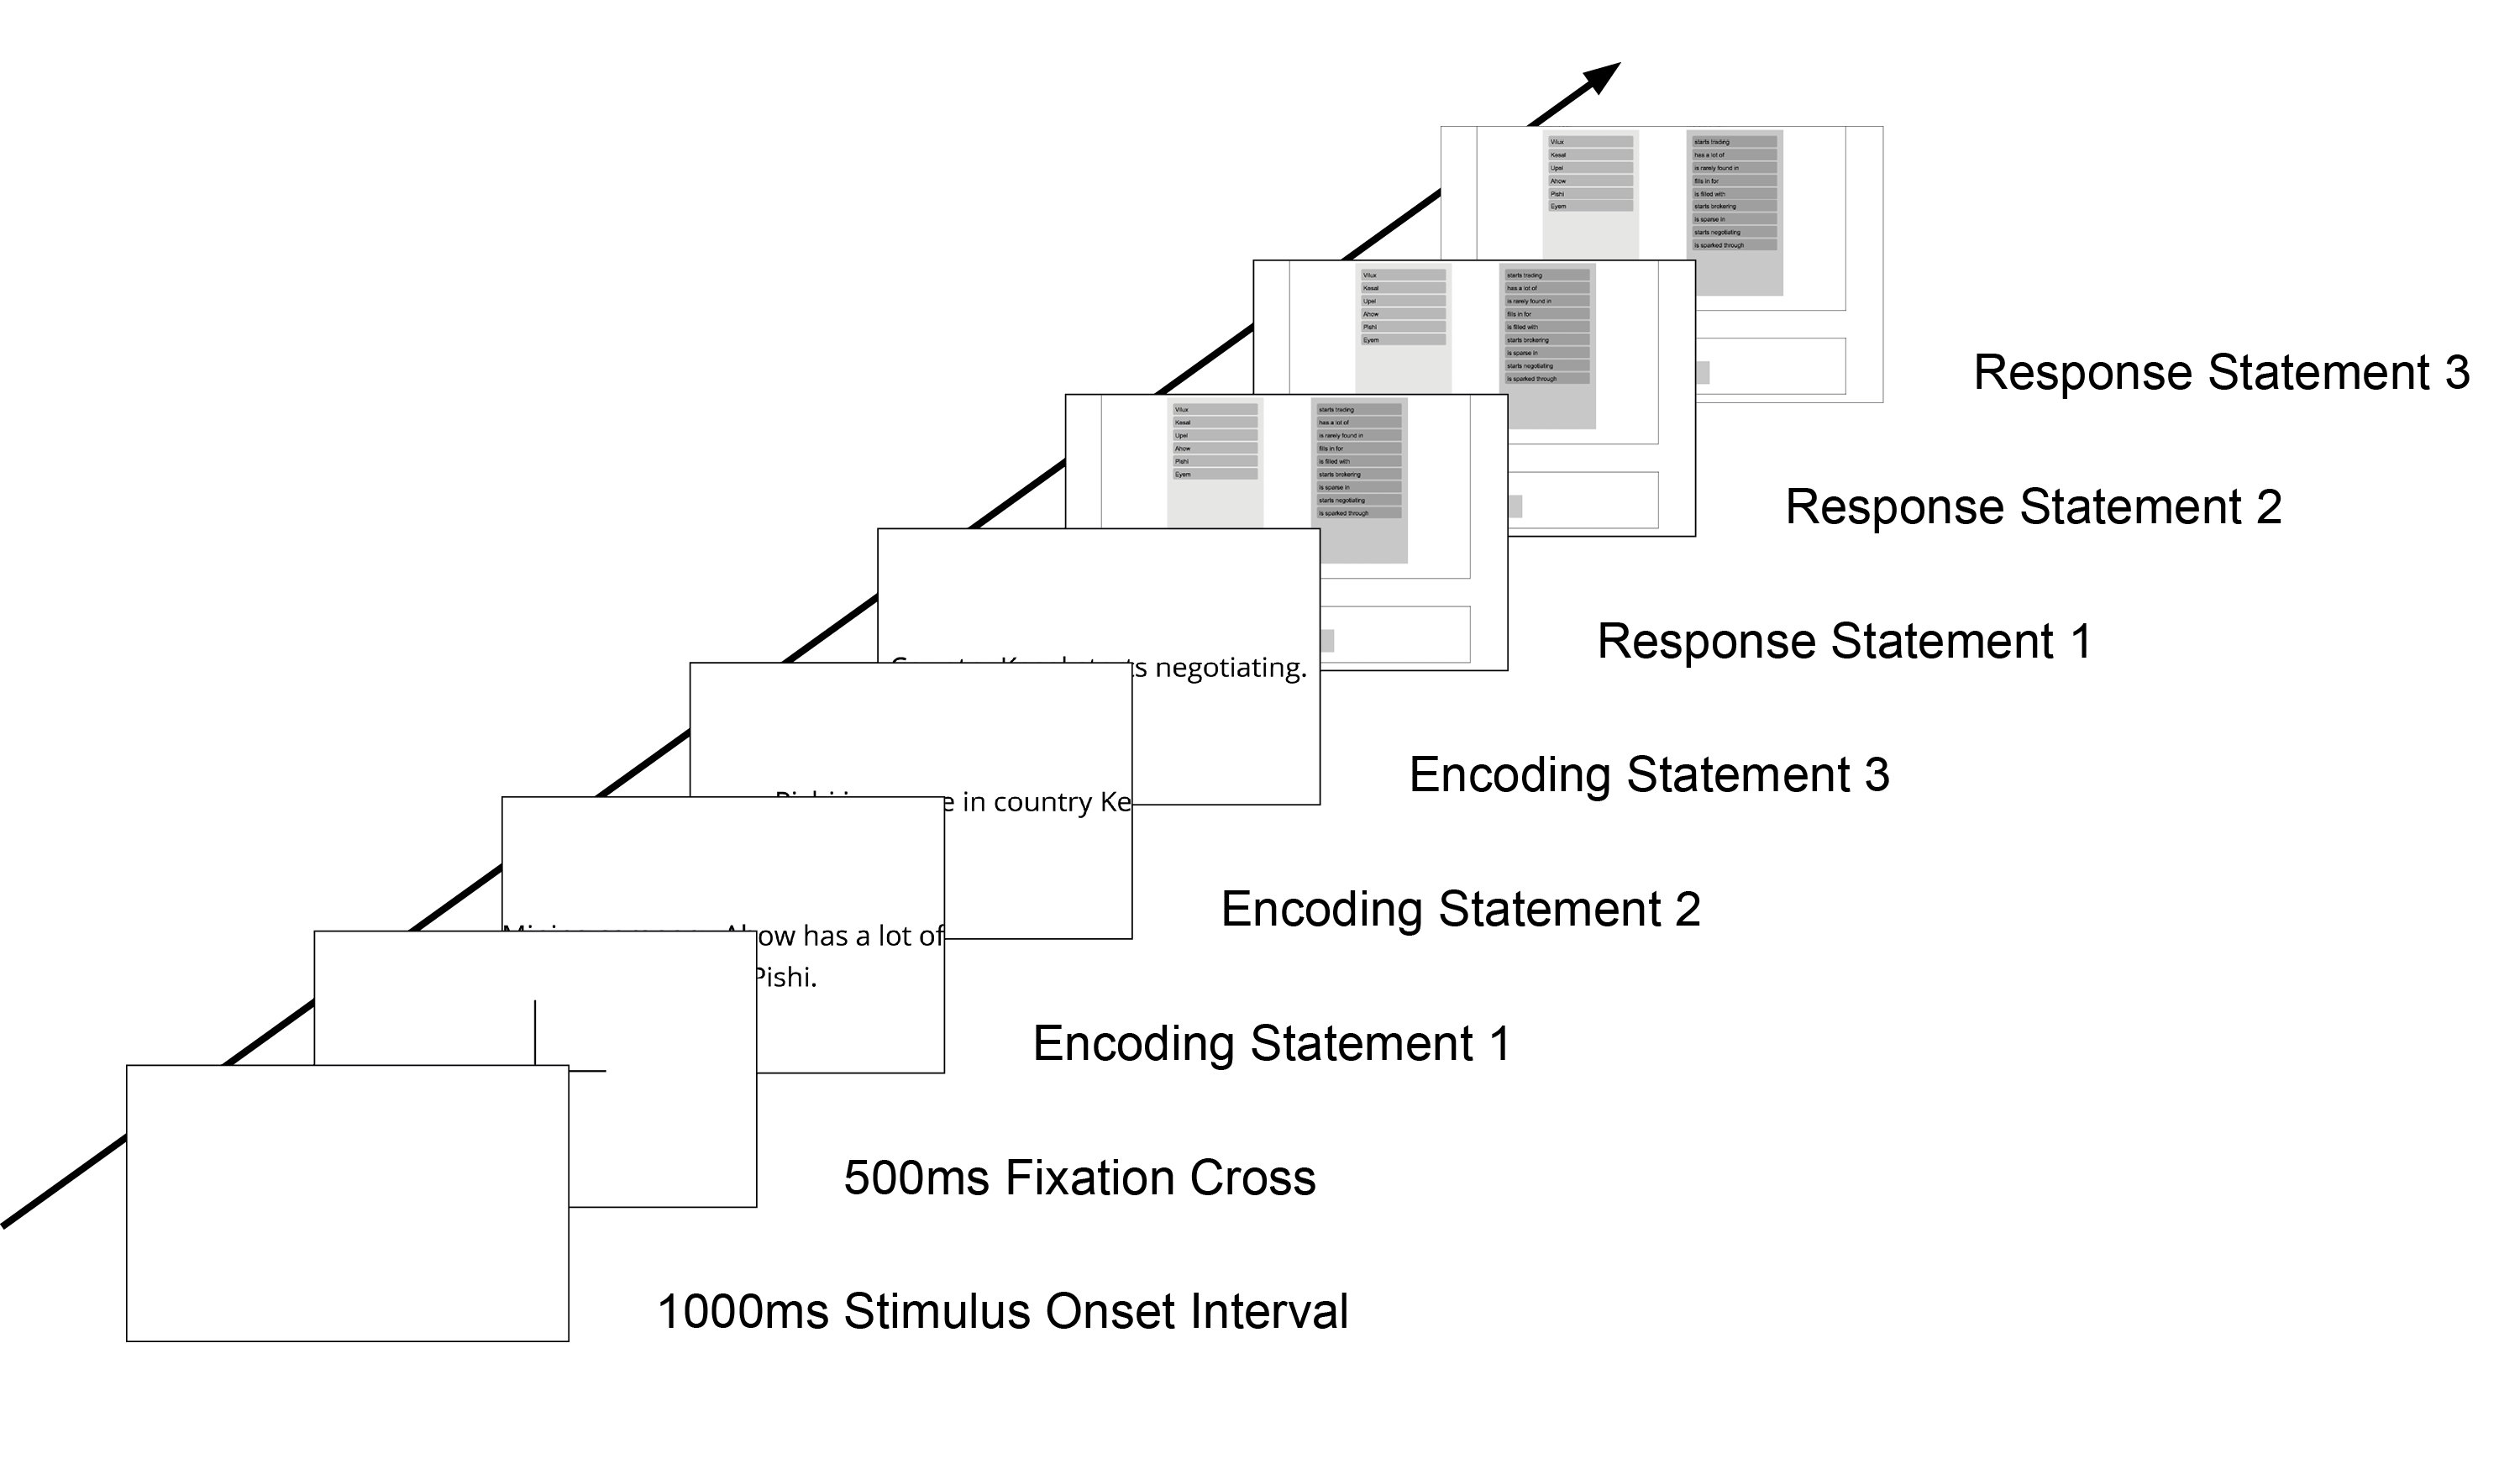
\includegraphics[width=\textwidth]{figures/trial_sequence.png}
\caption{Sequence of a single trial.}
\label{fig:trial_sequence}
\end{center}
\end{figure}

\subsubsection{Participants}
For data collection we collected 109 observations from the online labour platform CrowdFlower. In the description of the task on CrowdFlower we explicitly asked for native english speaker, and set the country parameter on CrowdFlower to United States only. Nonetheless a few participants responded with different native languages than english in our post experiment survey and were therefore excluded from further analysis. In addition, 17 participants didn't pass the trick story, where they were supposed to recall a single statement (2 names and one relation) and where the response options offered 2 names and 3 relations. Those subjects were also excluded, which resulted in a sample of 85 subjects. Figure \ref{fig:sample_age} shows the sample's age distribution which varied between between 20 and 65 years old (median at 37), a rather wide age spectrum compared to traditional college student samples. The sample was equally distributed in terms of gender (50.3\% female). According to the self-reported highest degree of education, most of our sample had a university/college degree (58\%). Fewer had a high-school degree (39\%), and three subjects (3.6\%) reported having having a doctoral degree.

\begin{figure}
\begin{minipage}[t]{0.5\textwidth}
  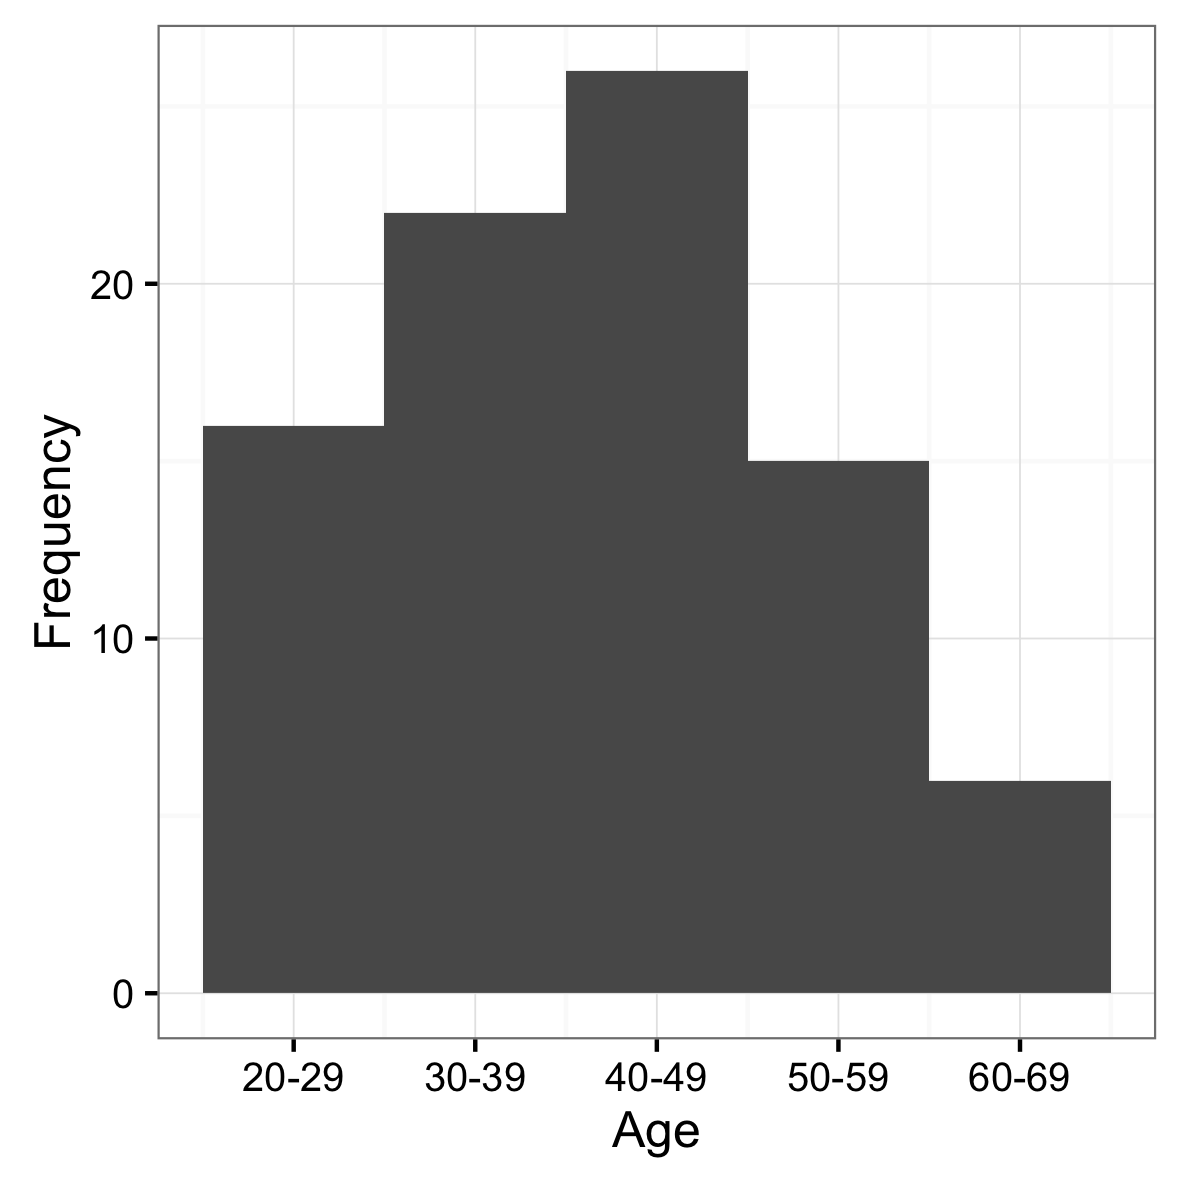
\includegraphics[width=.9\linewidth]{figures/sample_age.png}
  \caption{Distribution of age in the sample of experiment 1.}
  \label{fig:sample_age}
\end{minipage}
\begin{minipage}[t]{0.5\textwidth}
  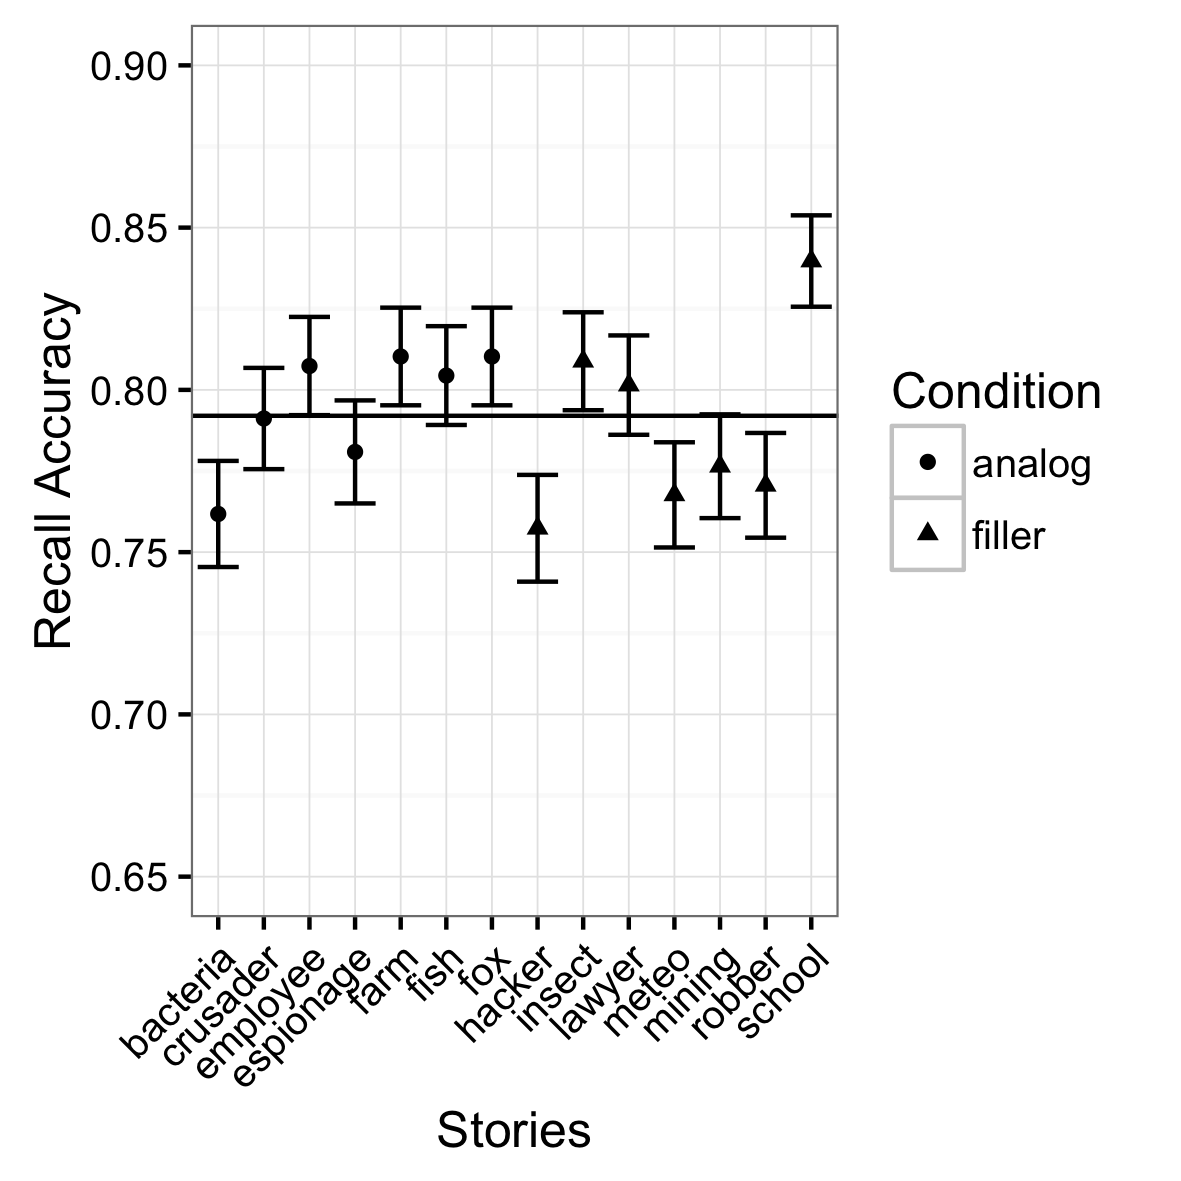
\includegraphics[width=.9\linewidth]{figures/material_stories.png}
  \caption{Mean recall accuracy and standard error for each story plus grand mean.}
  \label{fig:material_stories}
\end{minipage}
\end{figure}

\subsubsection{Material}
We constructed two sets of short analog and filler stories consisting of three statements each. The goal was to build all stories with a minimum of surface similarity overlap, i.e. no two stories with animals or where plumbers have a lead role. Three named entities were part of each story. To rule out individual differences in name recognition, and also to make the task more difficult, the names were randomly constructed by a free online service on dialectcreator.com so they were nonsensical. All analog stories had the following causal structure: "Entity A is responsible for entity B", "Entity B overcomes protection of entity C" and "Entity C endures negative consequence". The filler stories were constructed to be linguistically as similar as possible and therefore the sequence of relations and entities resembled the analog stories. The major difference between analog and fillers stories was the lack of systematicity when trying to map them on to each other, due to the lack of a shared higher order relational structure. To see the full table of stories and names see the appendix.
As response options we offered another alternative for each name, resulting in a total of 6 name-options per story, while only 3 of those appeared in the presented statements. For each relation from a story, we constructed two alternative response options, one was supposed to be synonymous to the correct relation, and one which was linguistically congruent but not in terms of the meaning. This resulted in a total of 9 relation options per story.
For each story we were recording 3 relation responses and 5 name responses (2+2+1 per statement), resulting in 9 items per story. We constructed 7 analog and 7 filler stories for this experiment. This gave us 85*14*8 = 9520 binary observations of recall success to work with.

\subsubsection{Procedure}
Participants had to open a link on CrowdFlower where they were sent to a webpage on our server on Openshift. We asked them to shut all other programs so they weren't disturbed by notifications. They were also reminded to put themselves in a quiet environment and reduce distractions like noise to a minimum. The experiment then launched into fullscreen mode and after giving consent and reading the instructions, the memory task was started. Alternately seven analog and filler stories were presented. The order within the analog and filler stories was randomized. Participants either started with an analog or a filler story, although we had to fix this part of randomization due to a bug after we started collecting data. Subjects starting with filler stories were therefore collected at another date. After the 12th story we injected a trick story consisting of only one statement and two names, to check if the participants were paying attention. As response options, only the two names which appeared in the previous statement and three relation options were presented. After the trick story, we resumed with alternating another set of analog and filler stories.

Following the memory task, a set of three closed yes or no questions regarding the conscious registration of different aspects of repetition were asked for, with the options to explain in an open format if participants responded yes to the closed question. The questions built up on each other, each being a little more specific about the repeated causal structure then the previous one. The first one asked if participants noticed any similarities between the stories, while the second one asked for repetiting elements between the stories and the third question explicitly mentioned the repeated analog/causal structure. See the appendix for exact wording of the questions.

Thereafter a set of questions regarding the demographics (age, gender, highest degree of education, native language) followed. Additionally we asked for the amount of effort on a four point Likert scale ("0 - none" / "1 - a little bit" / "2 - quite some / "3 - a lot"). We also asked if they completed the experiment in a serious manner and we therefore should use their data for analysis. We promised to give them the regular payment independently of their answer to this question. For the exact wording of the instructions used on CrowdFlower and in the experiment please see the appendix or the raw material on Github \citep{Oesch2016}. At the end of the experiment, every participant got a confirmation code, which they had to paste back into the form on CrowdFlower. After completion of the task Participants were paid one dollar for going through the whole experiment and received a bonus of another two dollars if they showed effort. The median of total experiment duration was 21 mins.
Due to continuous bug monitoring, data was collected over various dates.


\subsection{Results and Discussion}
The raw code of the scripts used for figures and analyses is online on Github \citep{Oesch2016}.

\subsubsection{Material Assessment}
Even though we tried each story to be equally difficult to memorize, when dealing with language material it is hard to neutralize a bias introduced by language. Figure \ref{fig:material_stories} indicates a certain difference regarding story difficulty, which is confirmed in an analysis of variance on item level, F(13,9506) = 2.303, p=0.005. It is therefore important that we account for this bias in further analyses with random intercepts.

\subsubsection{General Task Performance}
General recall accuracy was much higher than expected. A pilot study investigating suitable story length resulted in overall recall accuracies around 60\%. Median of overall recall accuracy in this experiment was at 83\% and over 30\% of our participants had recalled more than 90\% of items correctly. Figure \ref{fig:genper_overall} depicts the distribution of overall recall accuracies per subject. We mentioned in the instructions, that no means to facilitate this task were allowed, contrary to the pilot study, where we didn't emphasize this. Also, this time we incentivized subjects to put effort into the task so they will receive a bonus, which could have led subjects to cheat.

\begin{figure}
\begin{minipage}[t]{.5\textwidth}
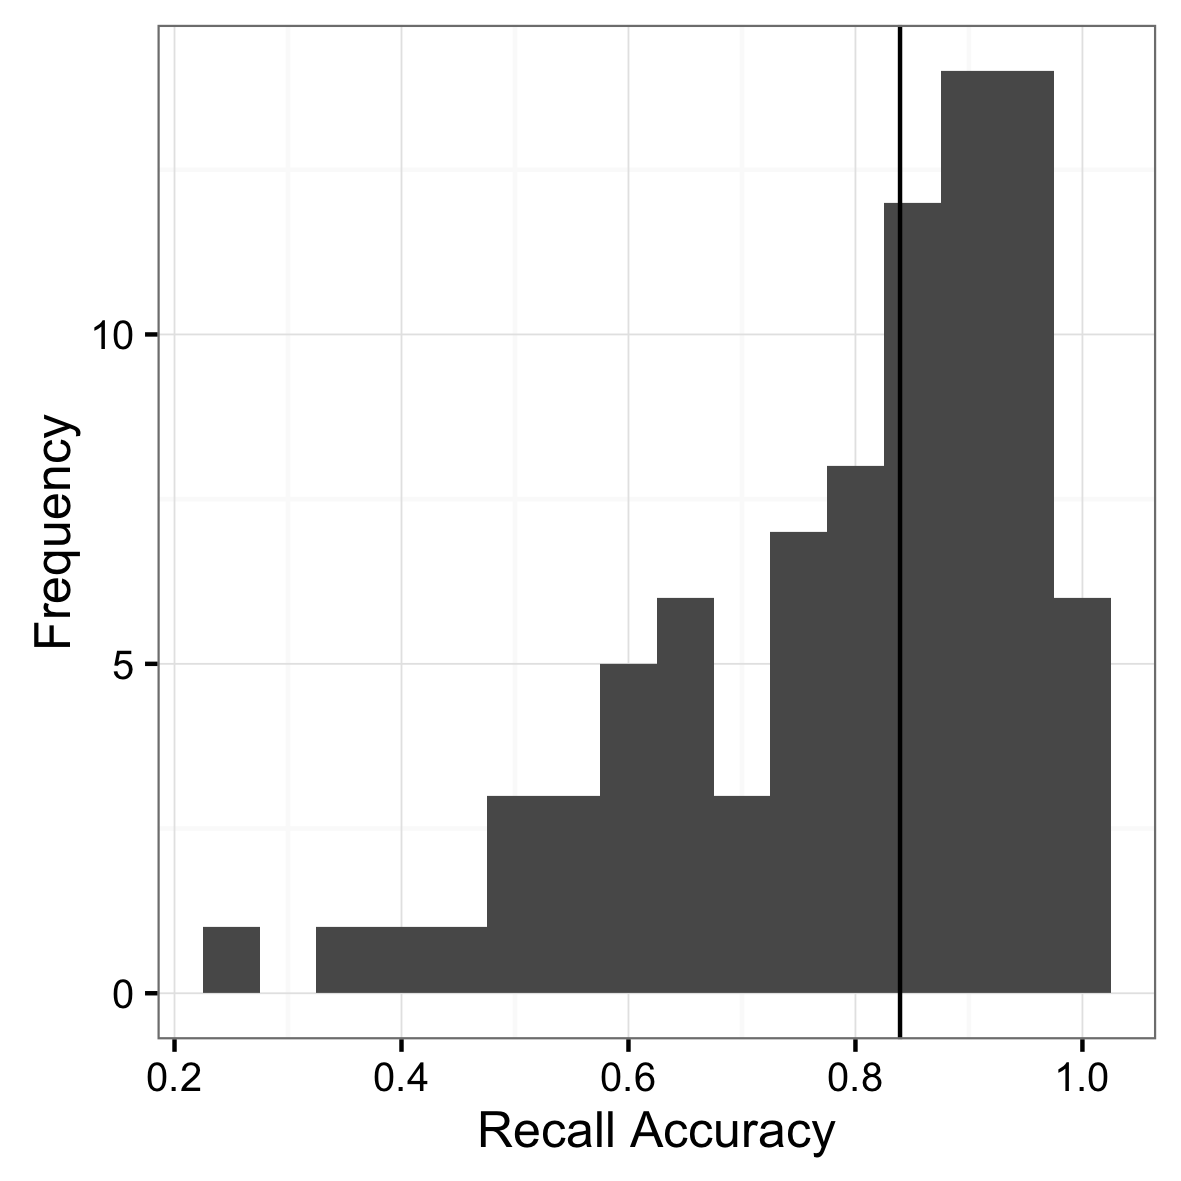
\includegraphics[width=.9\linewidth]{figures/genper_overall.png}
\caption{Distribution of overall recall accuracies per subject with median.}
\label{fig:genper_overall}
\end{minipage}
\begin{minipage}[t]{.5\textwidth}
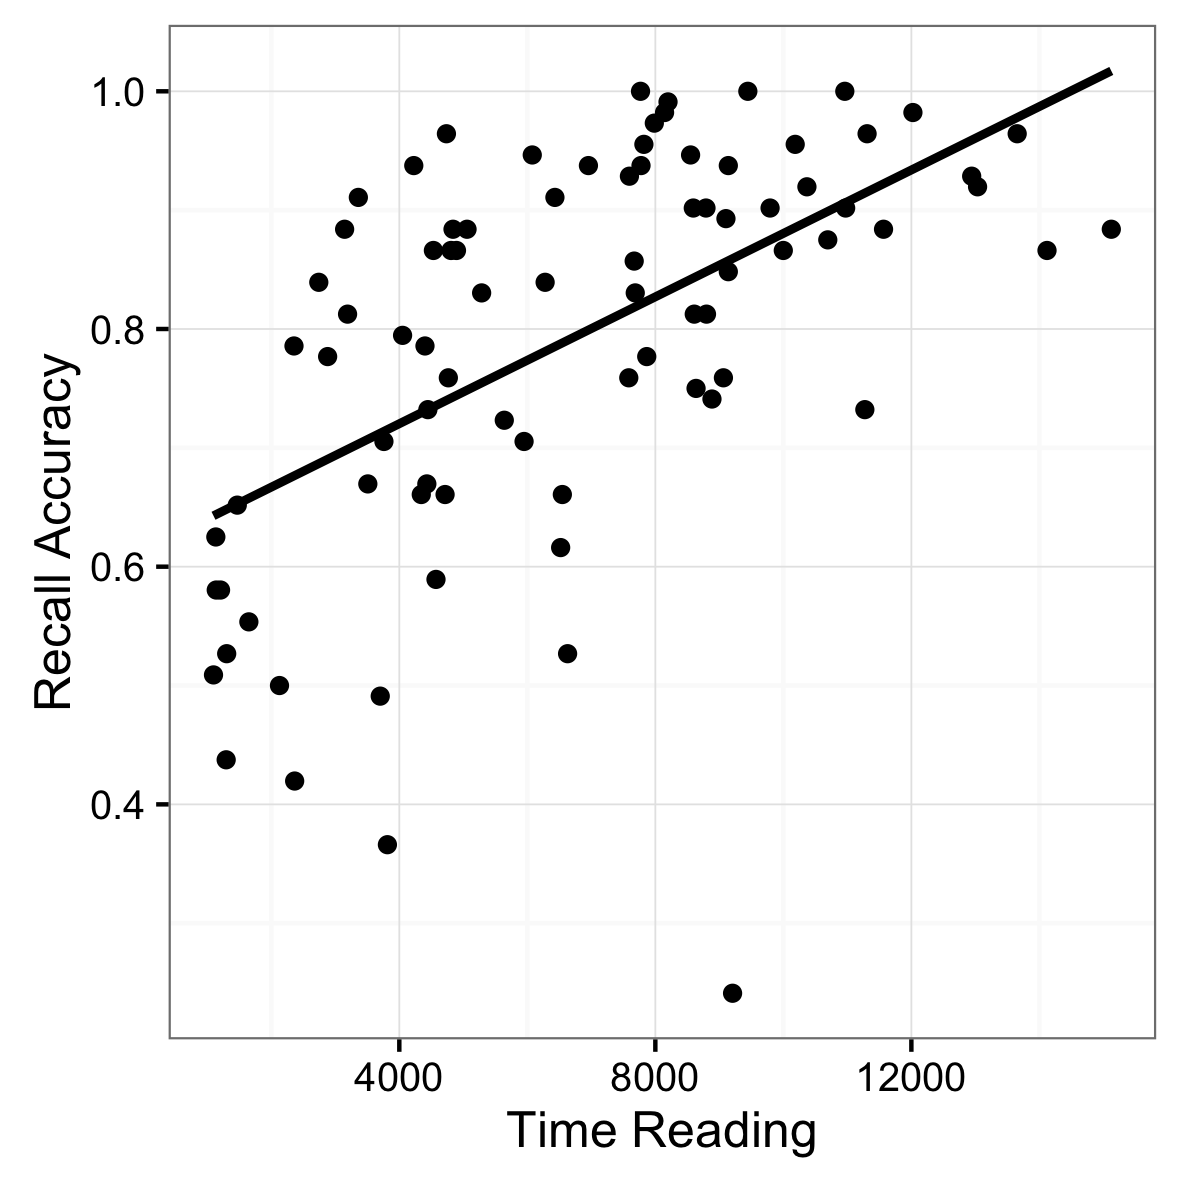
\includegraphics[width=.9\linewidth]{figures/genper_timeXoverall.png}
\caption{Correlation of subject's median statement reading time in milliseconds with overall recall accuracy.}
\label{fig:genper_timeXoverall}
\end{minipage}
\end{figure}


When comparing the median statement reading time per subject with the overall recall accuracies per subject (see Figure \ref{fig:genper_timeXoverall}), one can see an improved recall accuracy with increased median encoding time, the correlation is significant (\textit{r}(83) = 0.55, \textit{p} < 0.001). Half of our sample has a median of more than 6.5 seconds reading time for a single statement. This could be enough time to take notes (a little over 2 seconds per item), or just really put a lot of effort into encoding those two or three items and repeating the previous statement in a loop. Although when comparing self reported effort with recall accuracies then this does not seems not to have a big effect either on recall accuracy (see figure \ref{fig:genper_effortXoverall}) and encoding time (see Figure \ref{fig:genper_effortXtime}). An analyis of variance with recall accuracy as dependent variable and effort as independent variable was not significant (\textit{F}(1,83) = 0.24, \textit{p} = 0.626). The ANOVA with the subject's median reading time was neither significant (\textit{F}(1,83) = 0.83, \textit{p} = 0.364).

% phonetic loop would also mean more reading time with increased statement length.

\begin{figure}
\begin{minipage}[t]{.5\textwidth}
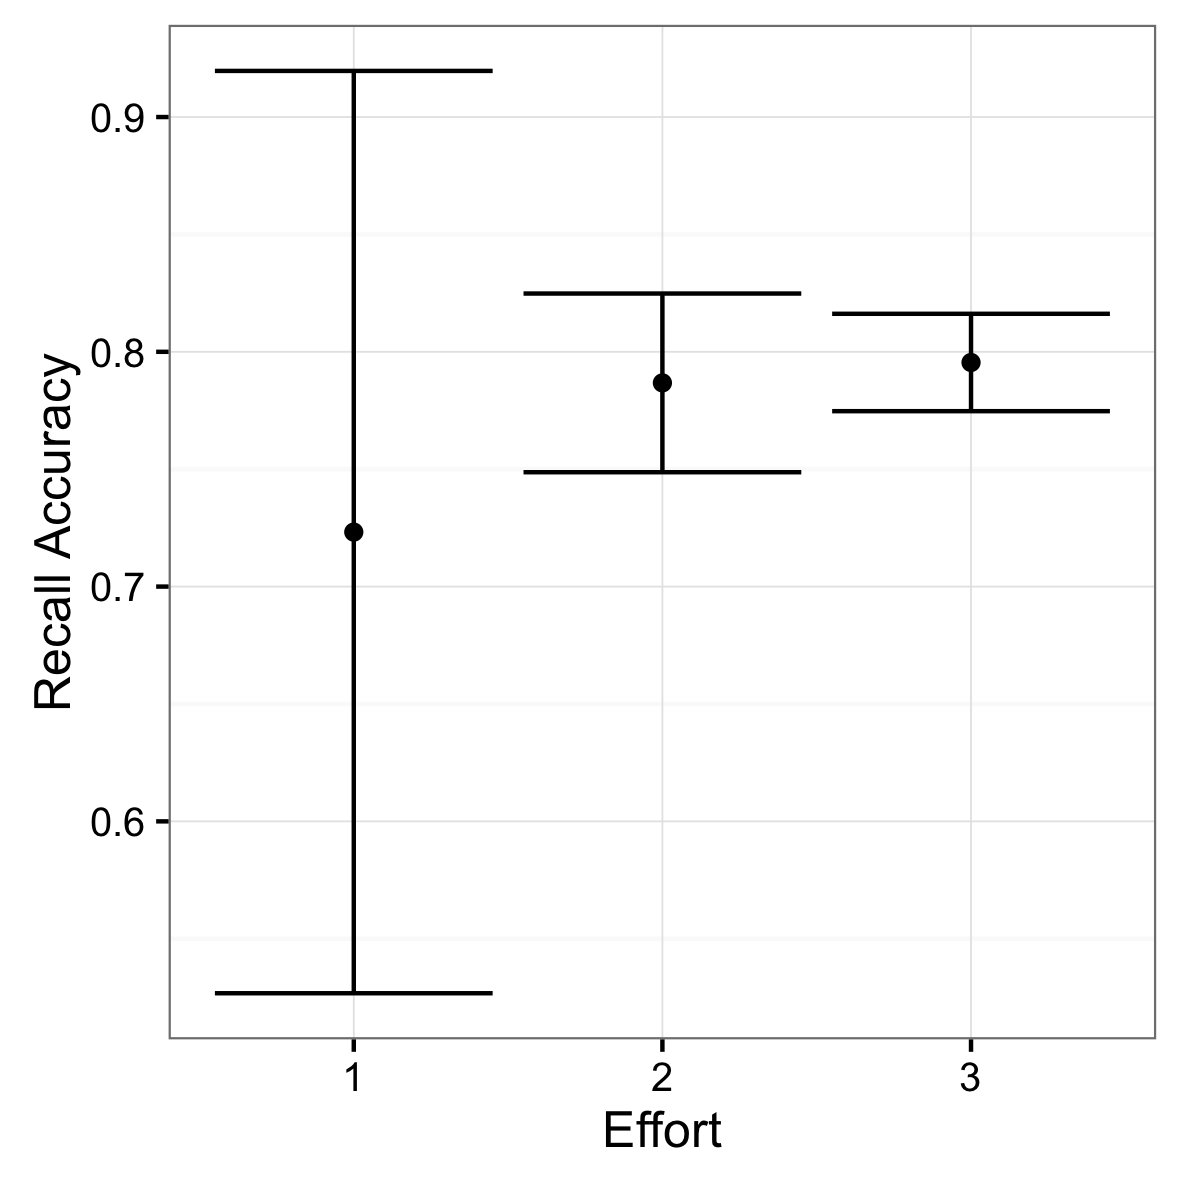
\includegraphics[width=.9\linewidth]{figures/genper_effortXoverall.png}
\caption{Self reported task effort on a 4-item Lickert scale (zeros removed) with mean and standard errors of recall accuracies per subject.}
\label{fig:genper_effortXoverall}
\end{minipage}
\begin{minipage}[t]{.5\textwidth}
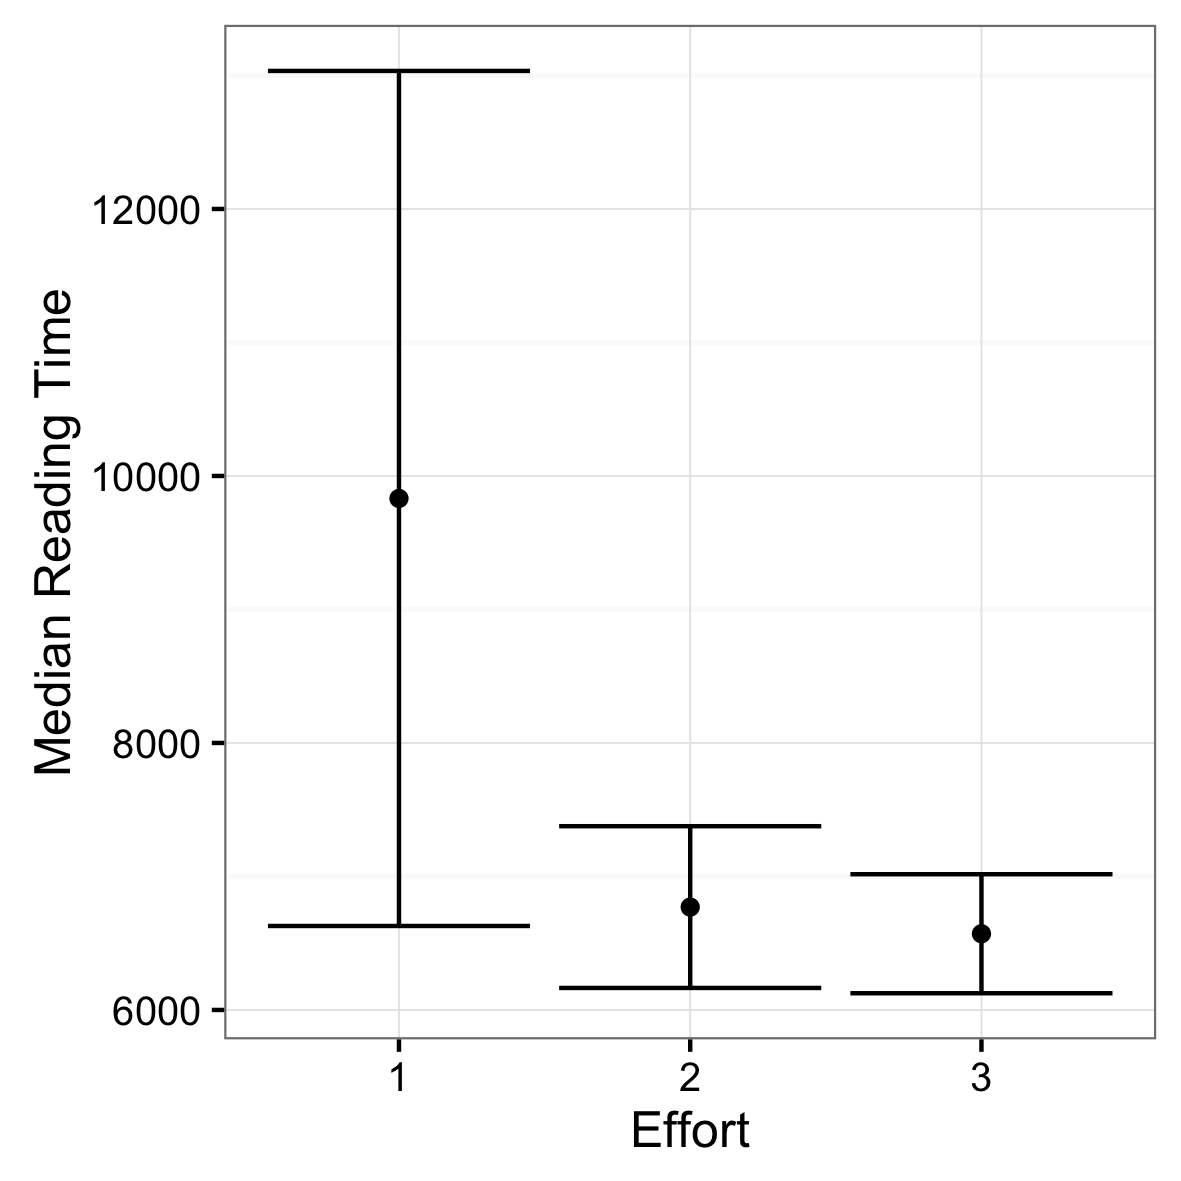
\includegraphics[width=.9\linewidth]{figures/genper_effortXtime.png}
\caption{Self reported task effort (see Fig. \ref{fig:genper_effortXoverall}) with mean and standard errors of per subject median reading time.}
\label{fig:genper_effortXtime}
\end{minipage}
\end{figure}


All in all those observations lead to the conclusion, that the task didn't reproduce a very natural reading and text comprehension environment. Participants did take a lot of time into encode or rehearse the items and we can not exclude the fact, that participants cheated by taking notes for example.

\subsubsection{Confounding Effects}
Nonetheless we could reproduce a set of well known effects from cognition literature with this setup, which legitimizes the interpretation of our results to a certain extent.

At first, we observed a general training effect as shown in figure \ref{fig:conf_stoidx}. A univariate logistic regression predicting recall success with the trial index is highly significant (\textit{e} = 0.043, \textit{z}(9518) = 7.321,  \textit{p} < 0.001). Although the trials 1 and 12 seem to deviate quite strongly from the general trend. It could be the case, that even though we presented participants with a pilot statement to give them the option the get accustomed to the response menu beforehand, participants didn't fully understand the task until after the first full trial. Further it should be noted that the trick story was inserted at the 11th trial position, but of course excluded from this analysis. Apparently the lack of coherence regarding story length confused participants remarkably and is observable in recall success.

\begin{figure}
\begin{minipage}[t]{.5\textwidth}
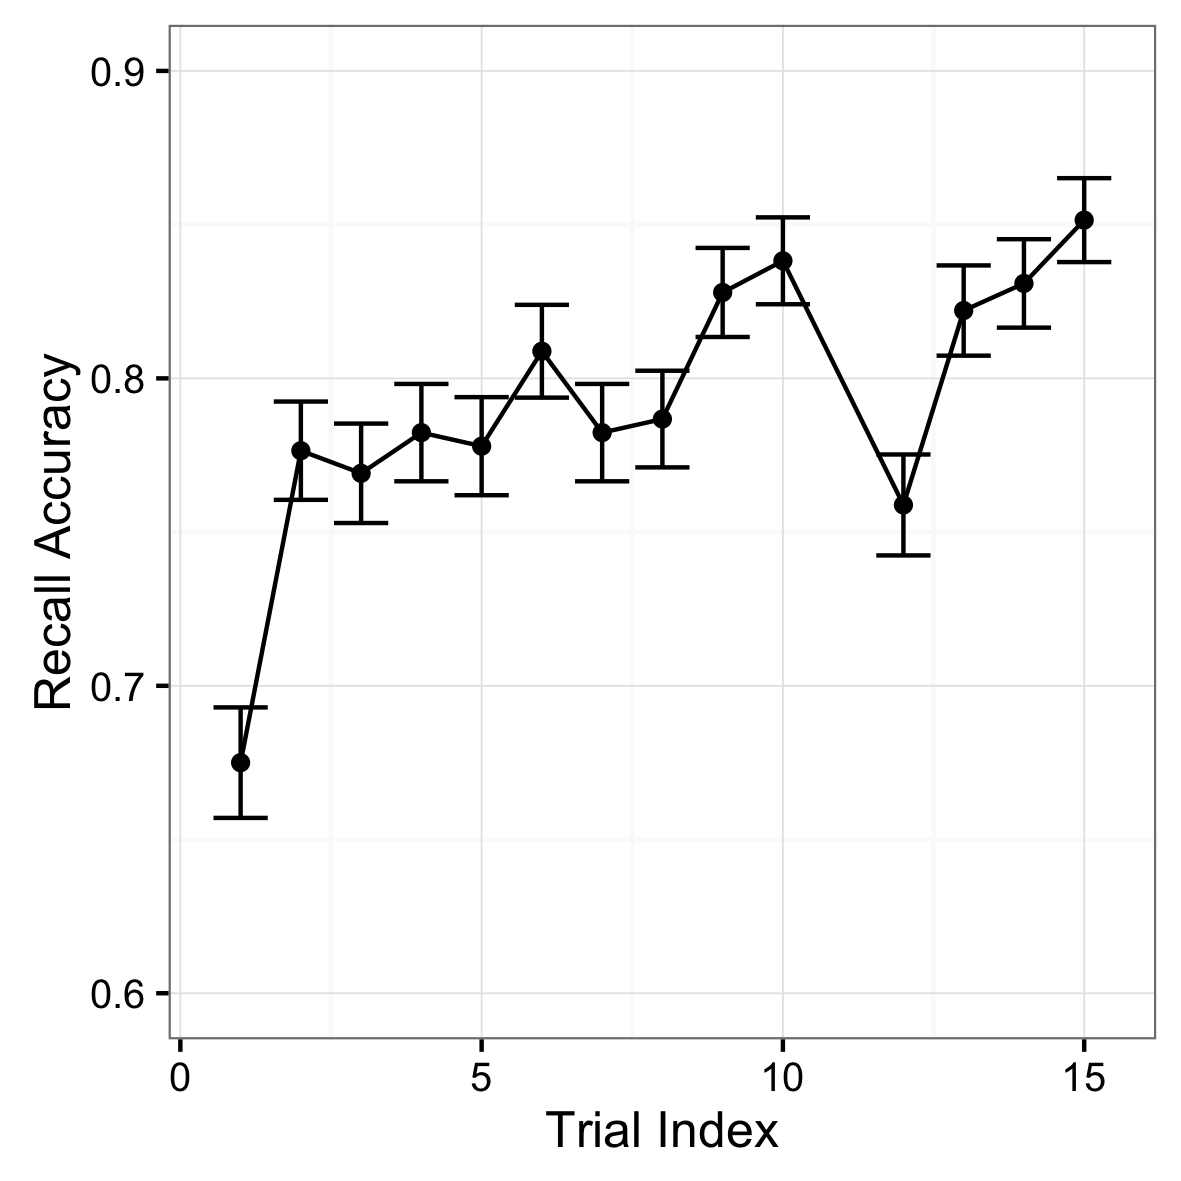
\includegraphics[width=.9\linewidth]{figures/conf_stoidx.png}
\caption{Mean recall accuracy and standard errors for each trial index.}
\label{fig:conf_stoidx}
\end{minipage}
\begin{minipage}[t]{.5\textwidth}
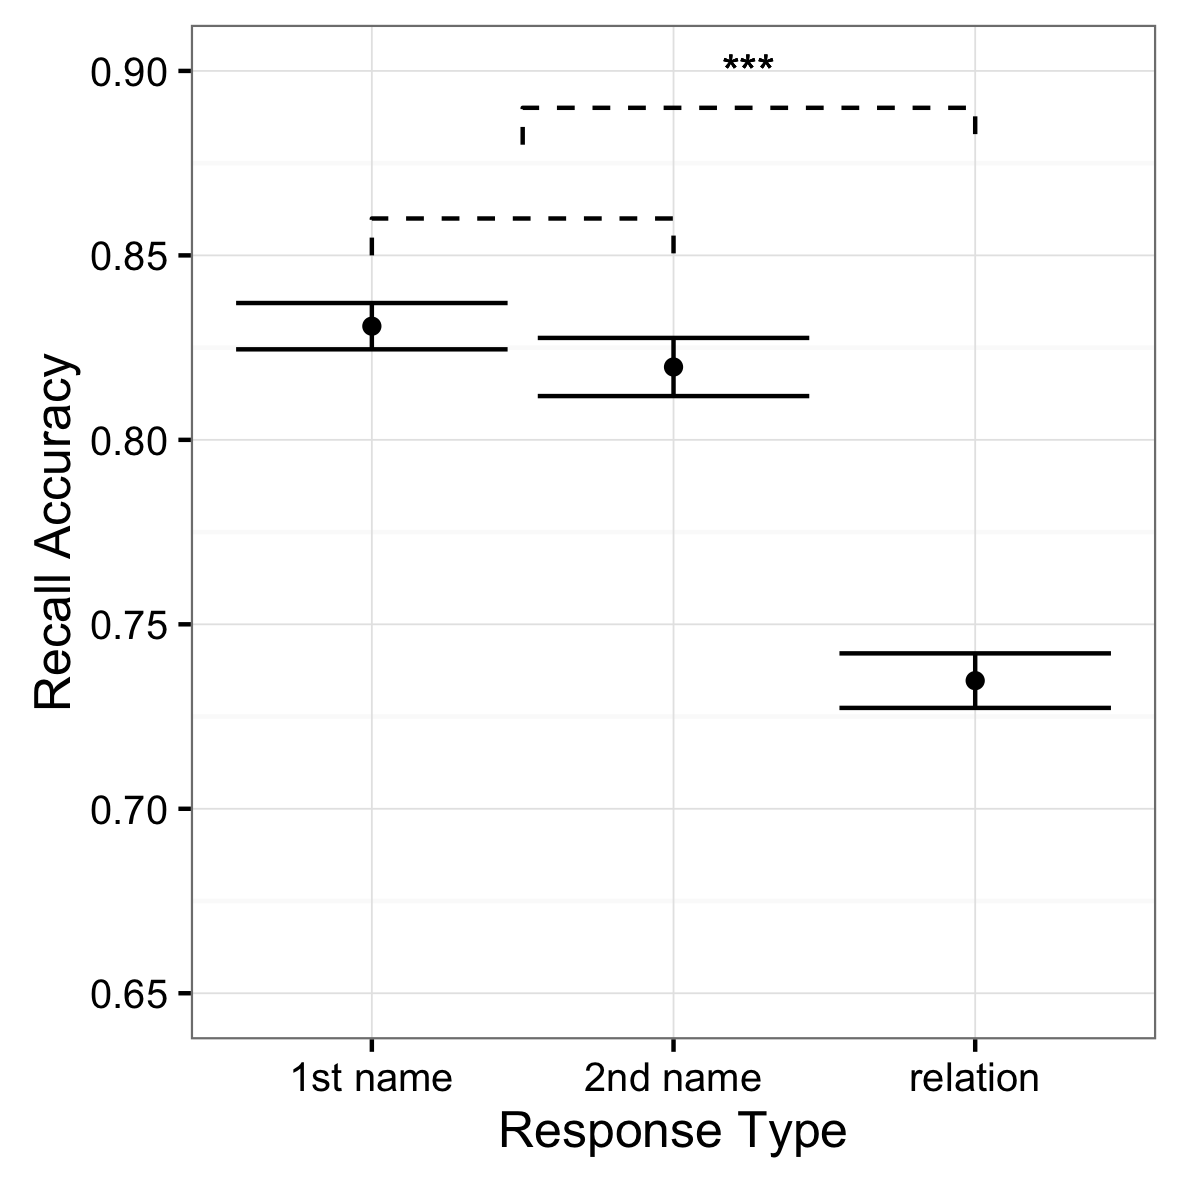
\includegraphics[width=.9\linewidth]{figures/conf_respType.png}
\caption{Mean recall accuracy and standard errors for each reponse type.}
\label{fig:conf_respType}
\end{minipage}
\end{figure}

Each statement had both entity names and relations. Figure \ref{conf_respType} depicts the difference in recall performance for each type of response item. The two different name responses did not differ significantly (\textit{${\chi}^2$}(1, \textit{N} = 5950) = 1.219, \textit{p} = 0.270 ), which is why we grouped both name responses together for further analyses. Relation items were significantly easier to recall (\textit{${\chi}^2$}(1, \textit{N} = 9520) = 113.78, \textit{p} < 0.001 ). This effect can most probably attributed to the nonsensicality of the names, which makes them harder to recall, but it can also be argued that participants had to recall 5 names while only 3 relations. Maybe storage resources weren't equally distributed, but we will not go further into this topic.

We already analyzed the influence of median reading times per subject and detected its effect on a subjects overall recall accuracy (see General Task Performance). Therefore it is not surprising to see, that also in an item level the simple logistic regression analysis, the regression coefficient from the logarithm of the statement's reading time is highly significant (\textit{e} = 0.519, \textit{z}(9518) = 18.88, p < 0.001).

\begin{figure}
\begin{minipage}[t]{.5\textwidth}
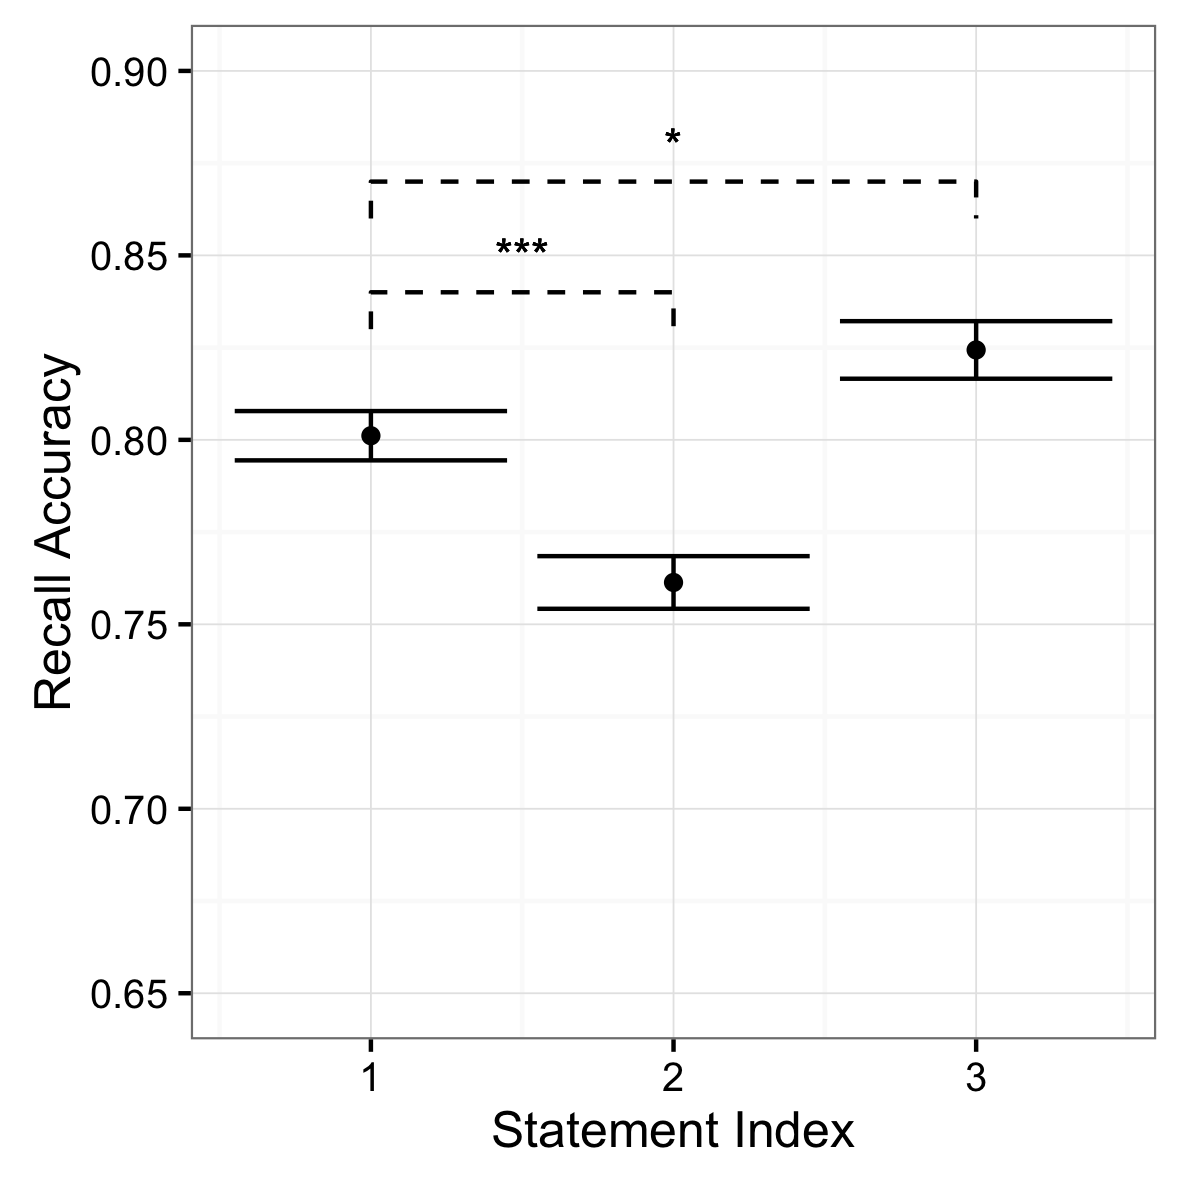
\includegraphics[width=.9\linewidth]{figures/conf_statIdx.png}
\caption{Mean recall accuracy and standard errors for each statement position.}
\label{fig:conf_statIdx}
\end{minipage}
\begin{minipage}[t]{.5\textwidth}
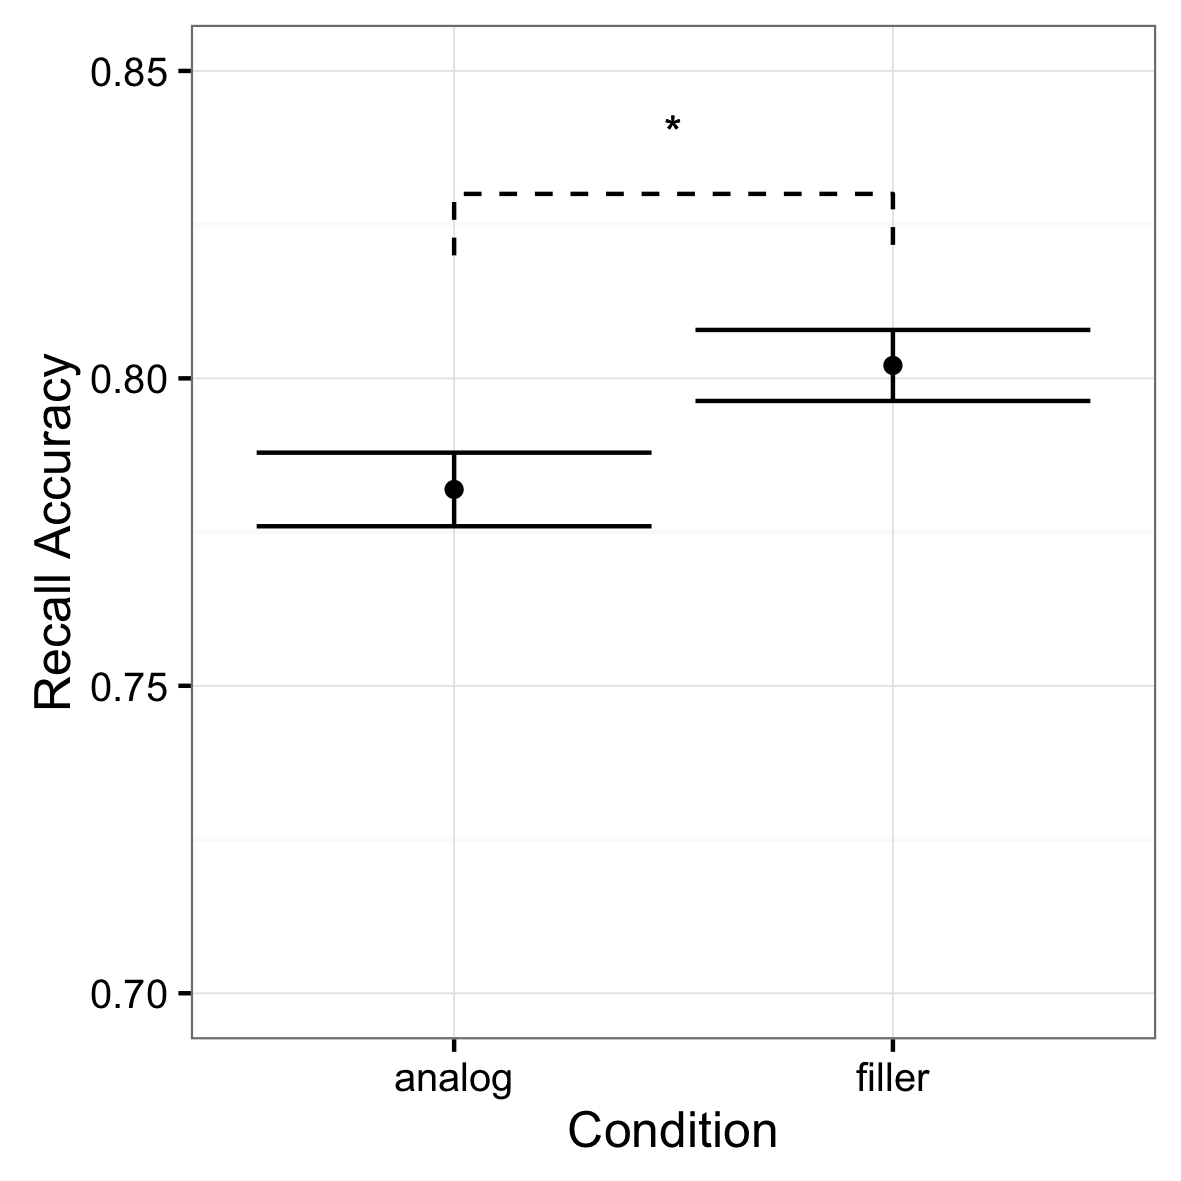
\includegraphics[width=.9\linewidth]{figures/conf_condition.png}
\caption{Mean recall accuracy and standard errors for each story structure condition.}
\label{fig:conf_condition}
\end{minipage}
\end{figure}

As each story had three statements, we were interested, if we can replicate a primacy and recency effect. Figure \ref{conf_statIdx} shows a clear difference in recall accuracy depending on the statements position in the story. A logistic regression predicting recall success with two dummy variables confirmed the statistical significance for the comparison second statement vs. first statement (\textit{e} = -0.233, \textit{z}(9517) = -4.06, \textit{p} < 0.001), and the comparison 3rd statement vs. 1st statement (\textit{e} = 0.153, (\textit{z}(9617) = 2.24, \textit{p} = 0.025). Although it should be noted, the second statement was linguistically the most complex, and the last statement in each story only had two items to remember. So it is not clear if the significant differences can be attributed to primacy/recency or rather to differing statement difficulties.

The two pools of stories we constructed, analog and fillers, only differed very slightly in terms of recall difficulty (see figure \ref{fig:conf_condition}). The mean of recall success only differs 2\% between the conditions. Nonetheless, due to the high statistical power the dummy variable comparing analog to filler items shows significance when analyzed with ${\chi}^2$-test (\textit{${\chi}^2$}(1, \textit{N} = 9520) = 5.877, \textit{p} = 0.015).

\subsubsection{Main Effect}
Our main hypothesis was that repeated causal structure will lead to increased memory performance. Figure \ref{fig:main} depicts the interaction of story structure condition and trial index. At first sight, it looks quite messy and not like a consistent trend. But one has to consider, that in this visualization there's still a lot of noise embedded in the form of confounding effects. We tested the interaction on statistical significance with a crossed random effects logistic regression analysis predicting recall success by adapting a method from \cite{Baayen2008}. Table \ref{table:main} shows an overview of the models tested with different confounding parameters. All models therein have a random intercept for each subject and each statement, accounting for random biases introduced by individuals and linguistic differences.

\begin{figure}
\centering
\begin{minipage}[t]{.5\textwidth}
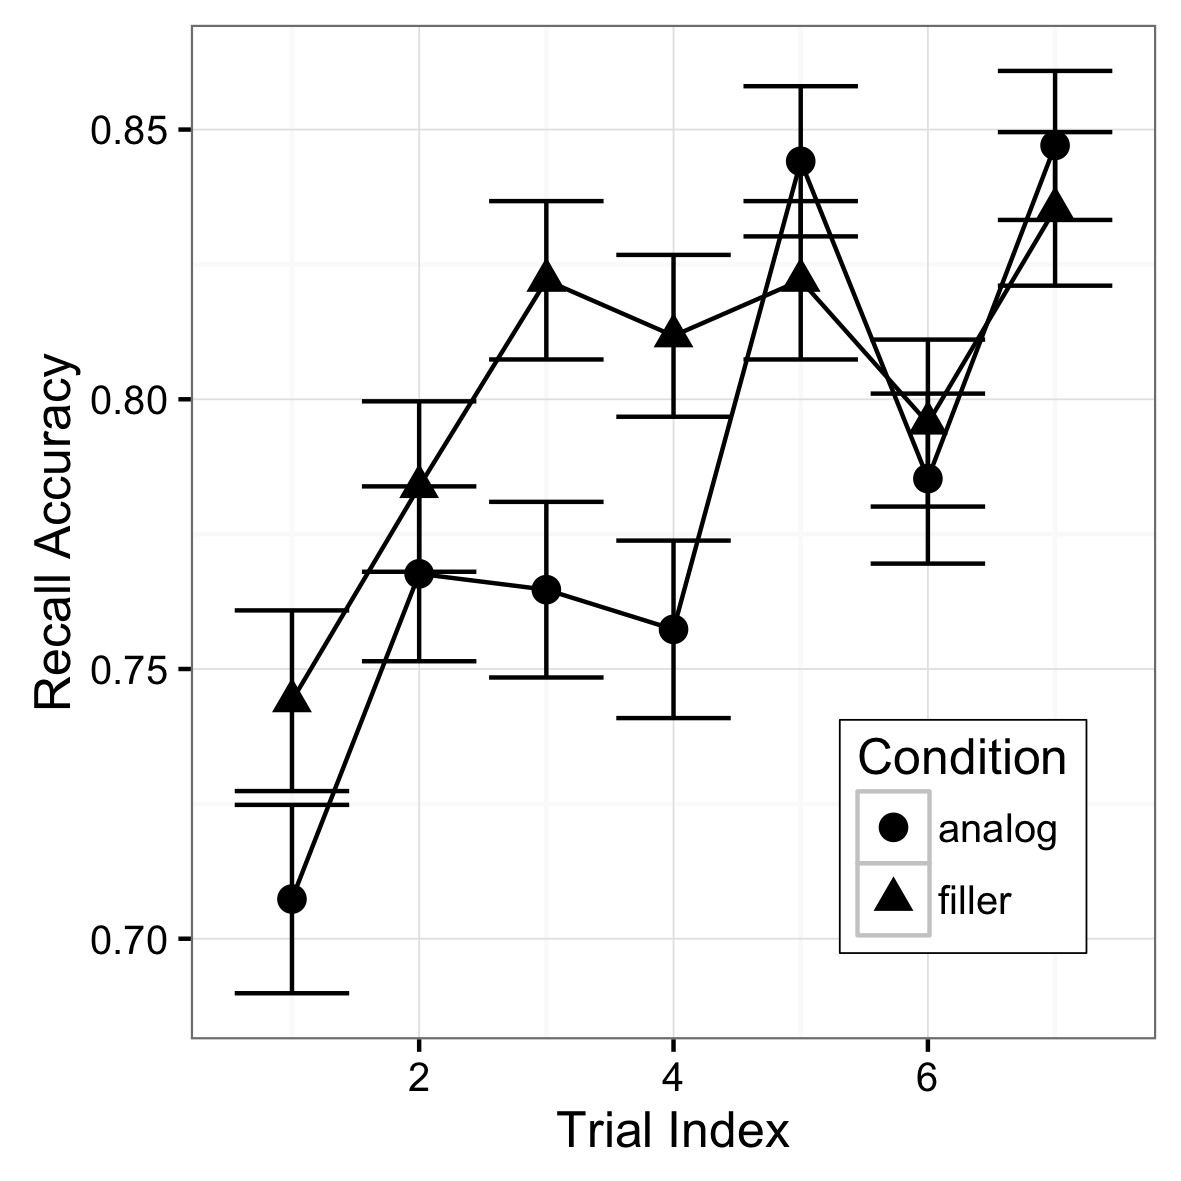
\includegraphics[width=.9\linewidth]{figures/main.png}
\caption{Mean recall accuracy and standard errors for each story position and story structure condition.}
\label{fig:main}
\end{minipage}
\end{figure}

All models from table \ref{table:main} are nested, which makes their log-likelihood comparable. The significance stars next to the log-likelihood indicates the significance level of the ${\chi}^2$-test comparing the respective model to the next simpler (the one to the left). To test the interaction, we z-transformed the variables trial index and condition (story structure: analog vs. filler).

Model 1 is the simplest, only accounting for the single effects plus their interaction, which is our main focus. Bear in mind that those models are crossed random effects models with random subject and statement intercepts. We can see that trial index has a strong effect on recall success, which has already been visible in the figures \ref{fig:main} and \ref{fig:conf_stoidx}. The interaction seems to be not too far off from significance but has not reached the 5\%-cutoff. Although when adding additional controlling parameters (as in model 2, 3 and 4), the main interaction become more and more significant mainly due to its increased estimate. As suspected, the fit of the models increases when controlling for the confounding effects. According to the ${\chi}^2$-tests the loss of degrees of freedom seem justified. it is noteworthy that the increase in fit is quite large when adding the log of the time reading (model 4), compared to the increase in fit when adding "Statement Nr" (model 3).

\begin{landscape}

% Table created by stargazer v.5.2 by Marek Hlavac, Harvard University. E-mail: hlavac at fas.harvard.edu
% Date and time: Thu, Aug 11, 2016 - 00:30:34
\begin{table}
\centering
  \caption{}
  \label{table:main}
\small
\renewcommand{\arraystretch}{0.45}
\begin{tabular}{@{\extracolsep{5pt}}lcccccc}
\\[-1.8ex]\hline
\hline \\[-1.8ex]
 & \multicolumn{6}{c}{\textit{Dependent variable:}} \\
\cline{2-7}
\\[-1.8ex] & \multicolumn{6}{c}{Recall Sucess} \\
\\[-1.8ex] & (1) & (2) & (3) & (4) & (5) & (6)\\
\hline \\[-1.8ex]
 Trial Index & 0.218$^{**}$ & 0.223$^{**}$ & 0.222$^{**}$ & 0.280$^{**}$ & 0.327$^{**}$ & 0.256$^{**}$ \\
  & (0.028) & (0.028) & (0.028) & (0.029) & (0.031) & (0.034) \\
  & & & & & & \\
 Condition & 0.071 & 0.073 & 0.072$^{*}$ & 0.076$^{*}$ & 0.071$^{o}$ & 0.069$^{o}$ \\
  & (0.045) & (0.051) & (0.036) & (0.038) & (0.038) & (0.037) \\
  & & & & & & \\
 Response Type Relation &  & $-$0.703$^{**}$ & $-$0.724$^{**}$ & $-$0.738$^{**}$ & $-$0.740$^{**}$ & $-$0.743$^{**}$ \\
  &  & (0.057) & (0.057) & (0.058) & (0.058) & (0.058) \\
  & & & & & & \\
 Statement Nr 2 &  &  & $-$0.289$^{**}$ & $-$0.022 & $-$0.023 & $-$0.023 \\
  &  &  & (0.083) & (0.092) & (0.090) & (0.088) \\
  & & & & & & \\
 Statement Nr 3 &  &  & 0.311$^{**}$ & 0.938$^{**}$ & 0.941$^{**}$ & 0.943$^{**}$ \\
  &  &  & (0.093) & (0.113) & (0.112) & (0.110) \\
  & & & & & & \\
 Log Reading Time &  &  &  & 0.542$^{**}$ & 0.544$^{**}$ & 0.545$^{**}$ \\
  &  &  &  & (0.048) & (0.048) & (0.048) \\
  & & & & & & \\
 After Trick &  &  &  &  & $-$0.566$^{**}$ & $-$0.535$^{**}$ \\
  &  &  &  &  & (0.112) & (0.112) \\
  & & & & & & \\
 First &  &  &  &  &  & $-$0.547$^{**}$ \\
  &  &  &  &  &  & (0.110) \\
  & & & & & & \\
 Trial Index:Condition & $-$0.052$^{o}$ & $-$0.053$^{o}$ & $-$0.055$^{o}$ & $-$0.057$^{*}$ & $-$0.063$^{*}$ & $-$0.057$^{*}$ \\
  & (0.028) & (0.028) & (0.028) & (0.029) & (0.029) & (0.028) \\
  & & & & & & \\
 Constant & 1.726$^{**}$ & 2.036$^{**}$ & 2.051$^{**}$ & $-$2.838$^{**}$ & $-$2.810$^{**}$ & $-$2.780$^{**}$ \\
  & (0.139) & (0.146) & (0.149) & (0.449) & (0.449) & (0.449) \\
  & & & & & & \\
\hline \\[-1.8ex]
Observations & 9,520 & 9,520 & 9,520 & 9,520 & 9,520 & 9,520 \\
Log Likelihood & $-$4,191.375 & $-$4,116.757$^{***}$ & $-$4,101.298$^{***}$ & $-$4,030.975$^{***}$ & $-$4,018.804$^{***}$ & $-$4,006.802$^{***}$ \\
Akaike Inf. Crit. & 8,394.750 & 8,247.515 & 8,220.596 & 8,081.950 & 8,059.609 & 8,037.605 \\
Bayesian Inf. Crit. & 8,437.717 & 8,297.643 & 8,285.046 & 8,153.562 & 8,138.381 & 8,123.538 \\
\hline
\hline \\[-1.8ex]
\textit{Note:}  & \multicolumn{6}{r}{	\textsuperscript{o} p<0.1; * p<0.05; ** p<0.01; *** p<0.001} \\
\end{tabular}
\end{table}

\end{landscape}

To account for two anomalies in our data, we tested two additional models adding a free trial position parameter on each, the first parameter being "after trick". As we have seen in figure \ref{fig:conf_stoidx}, recall success remarkably declines after the insertion of the trick story in our trial sequence. To investigate the effect of this incoherence on our main interaction, we ran the logistic regression in model 5 with an extra free parameter for all trials after the trick story. Not surprisingly the log-likelihood of this model increases significantly, and the coefficient estimate for interaction is bigger then in the previous models.

The other anomaly from inspecting the effect of trial index on recall accuracy (fig. \ref{fig:conf_stoidx}) was the big deviation at the first trial. To investigate if the statistical power of the interaction mainly results from this deviation, we embedded another free parameter for all first trials. Even though we can observe a decreased coefficient estimate in the interaction in model 6, it stays below the 5\%-significance level.

\subsubsection{Reading Time}

\begin{figure}
\centering
\begin{minipage}[t]{.5\textwidth}
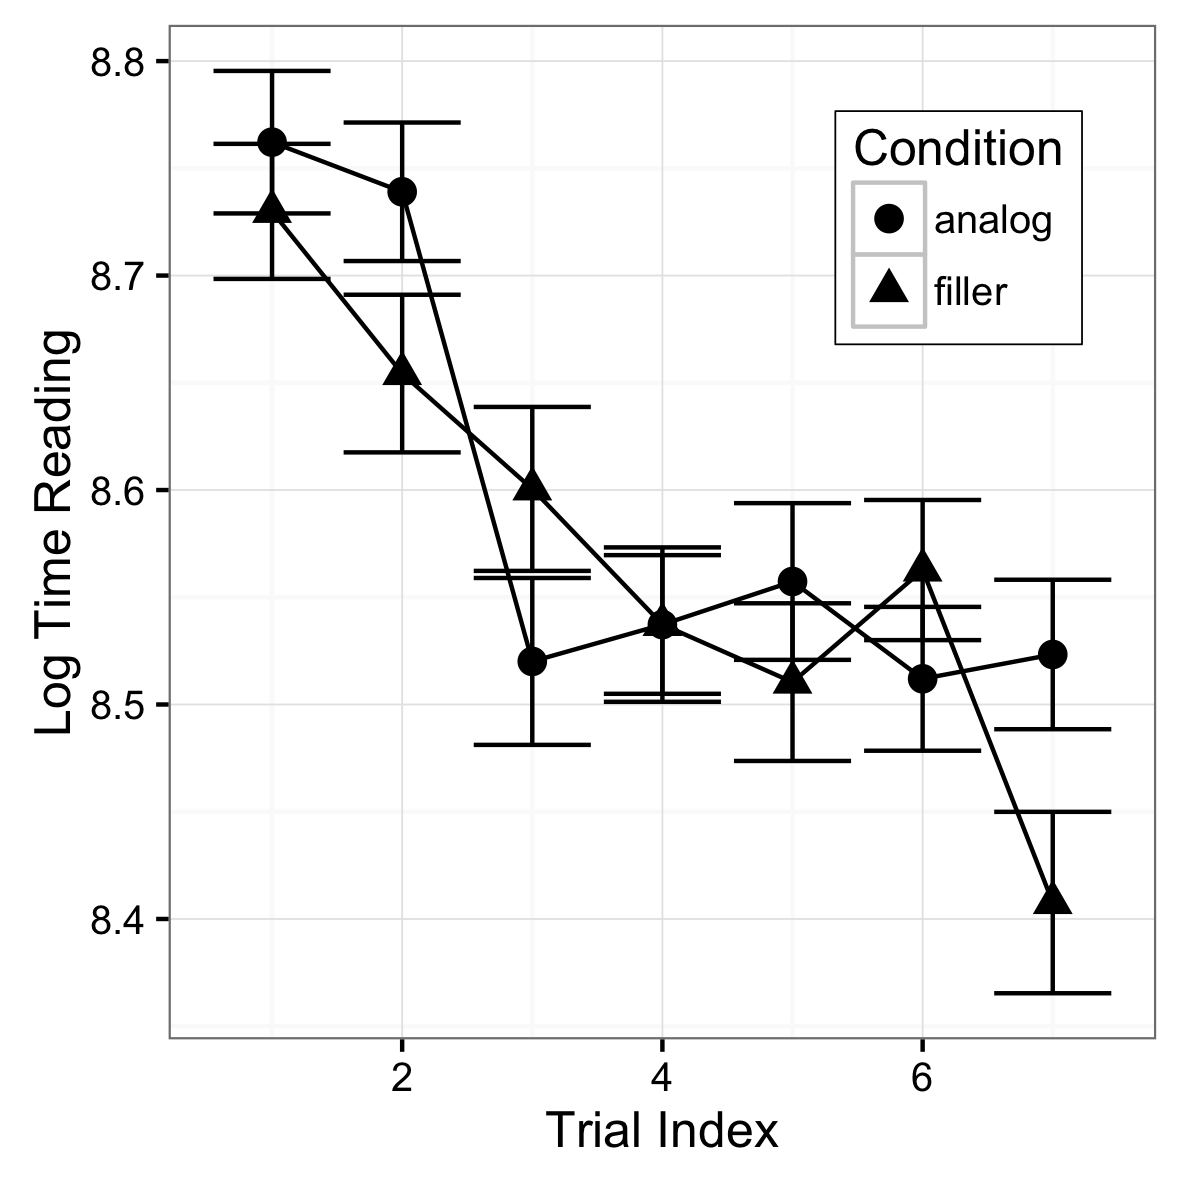
\includegraphics[width=.9\linewidth]{figures/read.png}
\caption{Mean and standard errors of the logarithm of the reading time in milliseconds for each trial index and story structure condition.}
\label{fig:read}
\end{minipage}
\end{figure}

\cite{Day2007} observed decreased encoding time when participants read a story which was structurally similar to the previous story. Therefore we also tested the effect of repeated causal structure on encoding time with a crossed random effects regression analysis, similar to when predicting recall success. This time it is not a logistic but a linear model. Also, the linear regression runs on the level of the statement (N=3570), and not item (N=9520). The interaction of story structure structure with trial index does not reach significance (see table \ref{table:read}). it is important to mention that our task crucially differed from \cite{Day2007} in the sense, that we specifically ask our participants to remember the different pieces of a very short story, while they have asked to actually comprehend a story with the expectation to answer questions about it. Also our material differs a lot in terms of complexity and conventionality.


% Table created by stargazer v.5.2 by Marek Hlavac, Harvard University. E-mail: hlavac at fas.harvard.edu
% Date and time: Thu, Aug 11, 2016 - 10:22:48
\begin{table} \centering
  \small
  \caption{Regression Coefficient and Standard Errors in Parentheses from Experiment 1}
  \label{table:read}
  \renewcommand{\arraystretch}{0.6}
\begin{tabular}{@{\extracolsep{5pt}}lcc}
\\[-1.8ex]\hline
\hline \\[-1.8ex]
 & \multicolumn{2}{c}{\textit{Linear Regression Models predicting the Logarithm of Time Reading:}} \\
\cline{2-3}
\\[-1.8ex] & (1) & (2)\\
\hline \\[-1.8ex]
 Trial Index & $-$0.082$^{**}$ & $-$0.082$^{**}$ \\
  & (0.010) & (0.010) \\
  & & \\
 Condition & $-$0.007 & $-$0.007 \\
  & (0.070) & (0.013) \\
  & & \\
 Statement Nr 2 &  & $-$0.422$^{**}$ \\
  &  & (0.032) \\
  & & \\
 Statement Nr 3 &  & $-$1.064$^{**}$ \\
  &  & (0.032) \\
  & & \\
 Trial Index:Condition & $-$0.004 & $-$0.004 \\
  & (0.010) & (0.010) \\
  & & \\
 Constant & 8.511$^{**}$ & 9.007$^{**}$ \\
  & (0.094) & (0.067) \\
  & & \\
\hline \\[-1.8ex]
Observations & 3,570 & 3,570 \\
Log Likelihood & $-$3,485.351 & $-$3,421.937$^{***}$ \\
Akaike Inf. Crit. & 6,984.703 & 6,861.874 \\
Bayesian Inf. Crit. & 7,027.965 & 6,917.497 \\
\hline
\hline \\[-1.8ex]
\textit{Note:}  & \multicolumn{2}{r}{	\textsuperscript{o} p<0.1; * p<0.05; ** p<0.01; *** p<0.001} \\
\end{tabular}
\end{table}


\subsubsection{Follow-Up}

\begin{figure}
\begin{minipage}[t]{.5\textwidth}
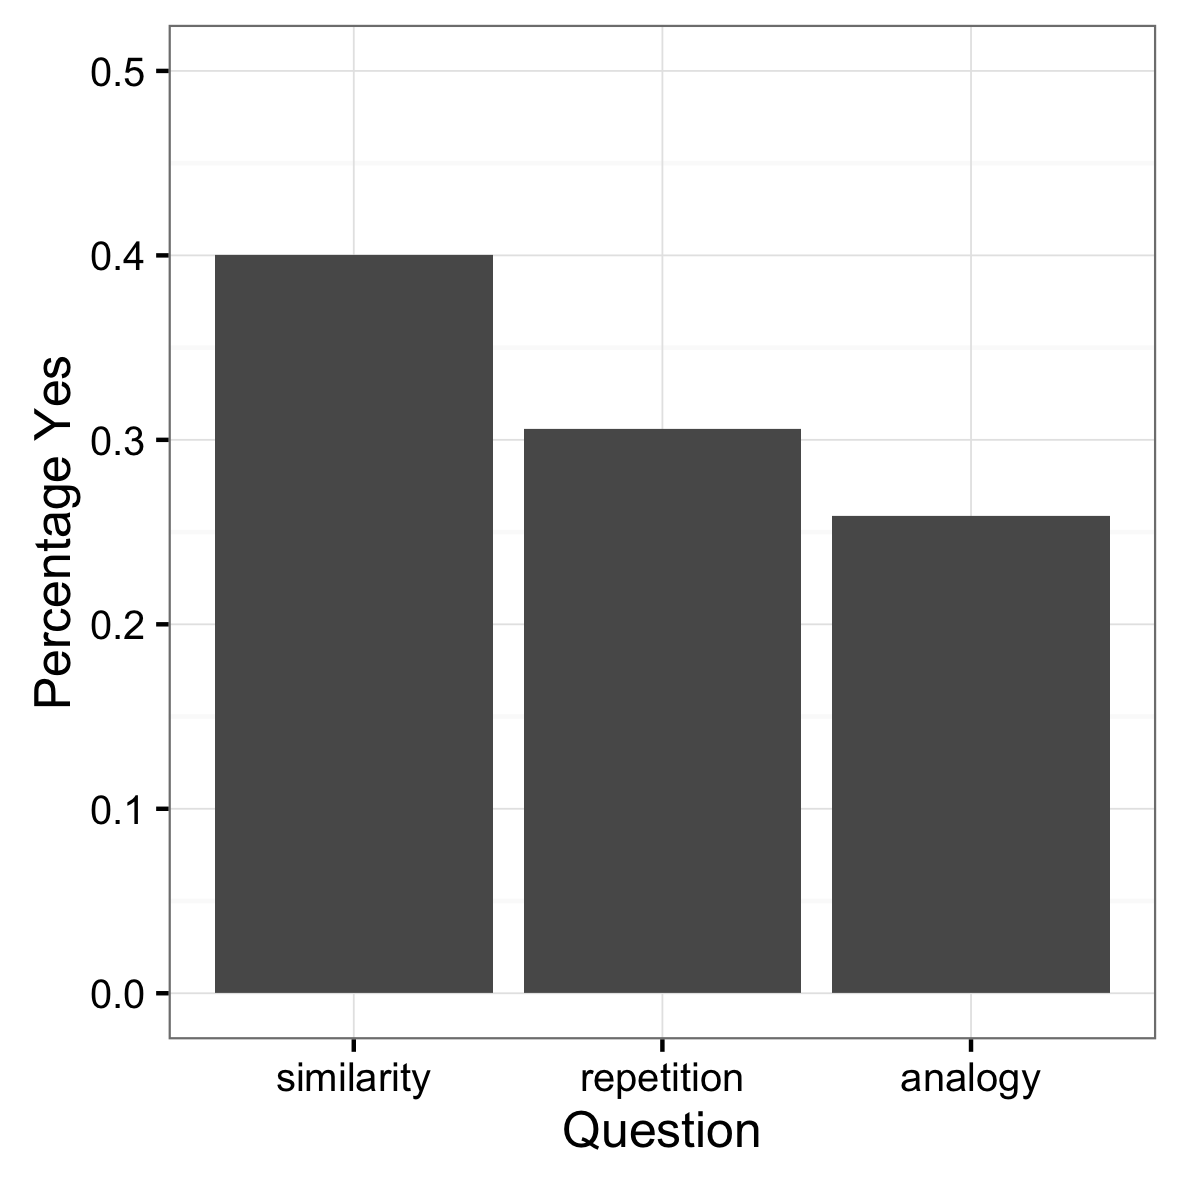
\includegraphics[width=.9\linewidth]{figures/fol_percYes.png}
\caption{Percentage of positive responses to the three follow-up questions.}
\label{fig:fol_percYes}
\end{minipage}
\begin{minipage}[t]{.5\textwidth}
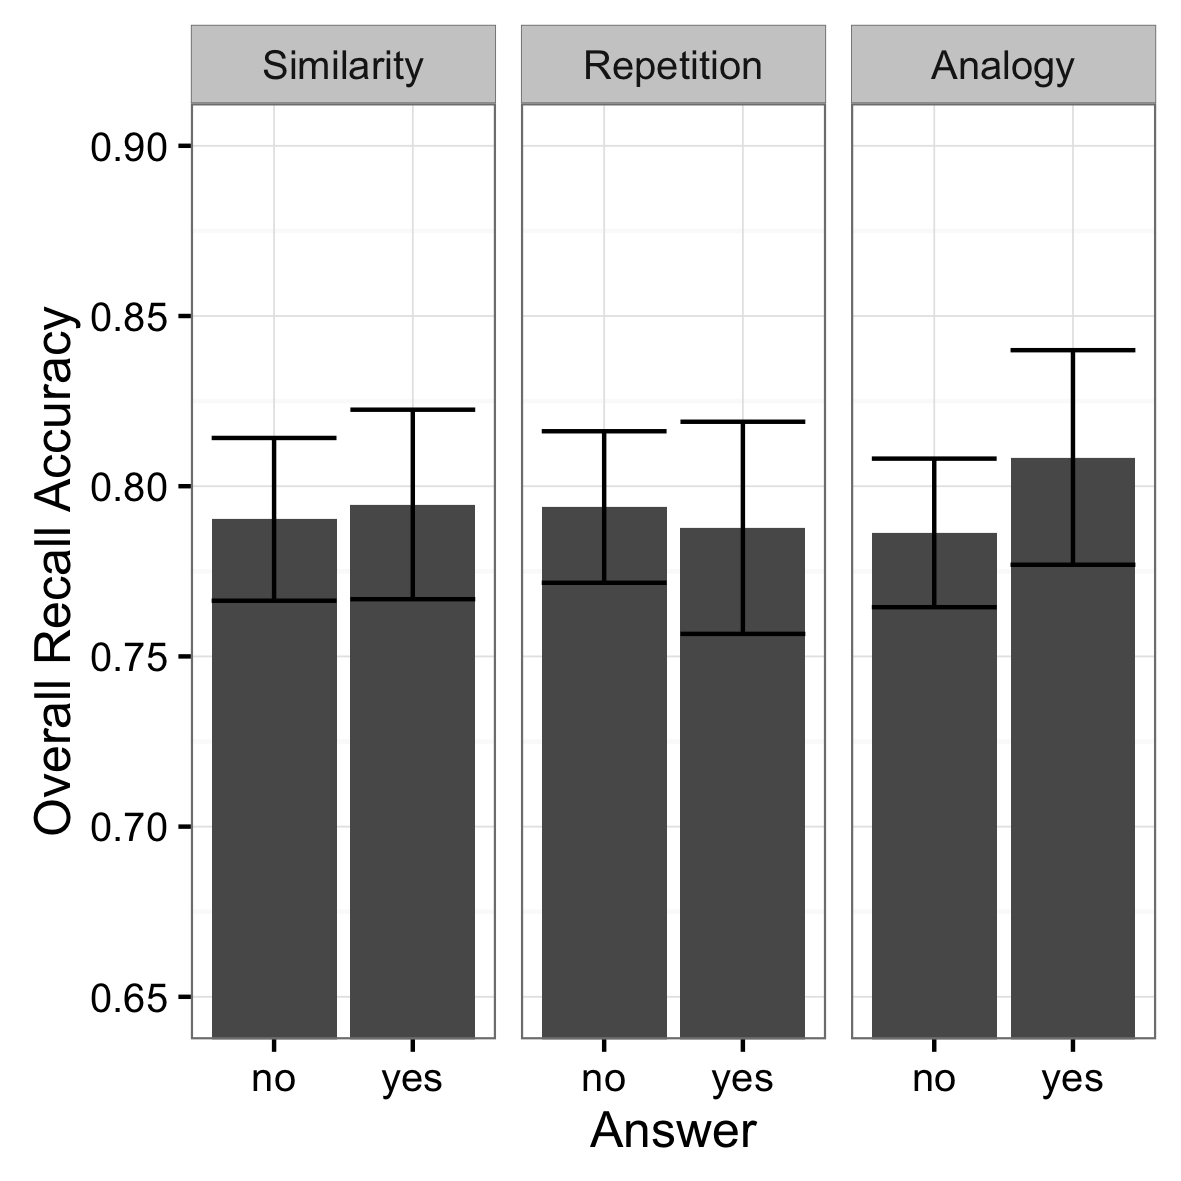
\includegraphics[width=.9\linewidth]{figures/fol_answerXoverall.png}
\caption{Mean and standard error of subjects overall recall accuracy for each response to the three follow-up questions.}
\label{fig:fol_answerXoverall}
\end{minipage}
\end{figure}

We claim that any analogical transfer in this experiment is unintentional, because participants are supposed to recall content and aren't told to explicitly compare stories to each other or even are aware of the systematicity. To check to what extent participants were aware of the repeated analog structure we asked three follow-up questions. The percentages of our sample that detected certain kinds of similarities between the stories are shown in figure \ref{fig:fol_percYes}. While 40\% reported to notice similarities between the stories, when asked to explain their response, most participants mentioned that all stories had nonsensical names. Some also mentioned the linguistic coherence ("Every story had 3 names of places, things or people.", "Every story had 2 actions and 1 consequence"). 31\% reported to having noticed repeating elements. The open answers were quite similar to the previous question. Only 26\% of our sample said to having noticed the repeating analog/causal structure in every second story. Although their open responses reveal, that often they meant the syntactic similarity instead of the causal structure. Only a very few participants really detected the repeating analog structure, indicating that most people could not have intentionally mapped stories on to each other.

We further investigated if detection of certain kinds of similarities between the stories had an effect on subject's overall recall accuracy. Figure \ref{fig:fol_answerXoverall} depicts those comparisons, which seem to not make a difference. Running simple linear regressions also showed no significant effect for any of the questions (see Table \ref{table:fol}), indicating that being aware of any kind of shared similarity did not yield any benefit in memory performance.


% Table created by stargazer v.5.2 by Marek Hlavac, Harvard University. E-mail: hlavac at fas.harvard.edu
% Date and time: Fri, Aug 12, 2016 - 20:54:33
\begin{table}[!htbp] \centering
  \caption{}
  \label{table:fol}
  \small
  \renewcommand{\arraystretch}{0.6}
\begin{tabular}{@{\extracolsep{5pt}}lccc}
\\[-1.8ex]\hline
\hline \\[-1.8ex]
 & \multicolumn{3}{c}{\textit{Dependent variable:}} \\
\cline{2-4}
\\[-1.8ex] & \multicolumn{3}{c}{Overall Recall Accuracy} \\
\\[-1.8ex] & (1) & (2) & (3)\\
\hline \\[-1.8ex]
 Similarity & 0.004 &  &  \\
  & (0.037) &  &  \\
  & & & \\
 Repetition &  & $-$0.006 &  \\
  &  & (0.039) &  \\
  & & & \\
 Analogy &  &  & 0.022 \\
  &  &  & (0.041) \\
  & & & \\
 Constant & 0.790$^{**}$ & 0.794$^{**}$ & 0.786$^{**}$ \\
  & (0.023) & (0.022) & (0.021) \\
  & & & \\
\hline \\[-1.8ex]
Observations & 85 & 85 & 85 \\
R$^{2}$ & 0.0002 & 0.0003 & 0.003 \\
Adjusted R$^{2}$ & $-$0.012 & $-$0.012 & $-$0.009 \\
Residual Std. Error (df = 83) & 0.167 & 0.167 & 0.167 \\
F Statistic (df = 1; 83) & 0.014 & 0.024 & 0.287 \\
\hline
\hline \\[-1.8ex]
\textit{Note:}  & \multicolumn{3}{r}{\textsuperscript{o} p<0.1; * p<0.05; ** p<0.01; *** p<0.001} \\
\end{tabular}
\end{table}


\subsection{Conclusion}
In this experiment we have discovered various weaknesses in the experimental setting. Nonetheless we could replicate a set of well known effects. Plus, there seems to be weak evidence for an increased learning rate with repeated causal structure. To strengthen our argument for analogical transfer in this hebb repetition paradigm, we decided to conduct another experiment, hoping to improve the methods where we see them unfit.

\newpage
\section{Experiment 2}
While in experiment 1 we only detected weak evidence for increased memory performance in repeated analogical structured stories, it could still be the case, that the effect is for example shadowed by the immediate change of story structure within the trial sequence. Opposed to relational priming studies, where the effect was usually observed when the same relation was activated just before the cued word pair. That's why we decided to investigate another experimental setting of immediate story structure repetition.
Another surprise in experiment 1 was the overall high recall success rate. We observed that participants were taking a lot of time to encode and/or rehearse the information. A lot more than would occur in a natural reading environment. We therefore decided to change the free reading time to a fixed time.
Due to the anomalies at trial position 1 and 11 in experiment 1, we also introduced a third category of stories, we called burn stories. These stories solely served the purpose of reducing noise from unintended trial sequence effects at the very beginning and after the trick story. They have the same characterization as the filler stories.

\subsection{Methods}
The methods were the same as in Experiment 1 with following exceptions.

\subsubsection{Task}
The task differed only regarding the fixed reading time. For each statement participants had 3 seconds to encode the information, which is less then half of the median time reading from experiment 1.

\subsubsection{Participants}
We again collected observations from 78 participants on Crowdflower. Applying the same exclusions criteria as in experiment 1, we ended up with a sample of 62 participants. Median age was 28 years, which is remarkably lower than in experiment 1 (see figure \ref{fig:sample2_age}). Qualification was equally balanced between high-school and university degrees (each 50\%). 60\% percent of our sample was female.


\begin{figure}
\centering
\begin{minipage}[t]{.9\textwidth}
\small
\begin{tabular}{| l | c | c | c | c | c | c | c | c | c | c | c | c | c | c | c | c | c |}
  \multicolumn{18}{c}{ }\\
  \hline
  \multicolumn{1}{| l }{Trial Sequences} & \multicolumn{17}{c |}{ } \\ \hline
  S1: & \cellcolor{black!10}B & \cellcolor{black!10}B & \cellcolor{black!10}B & \cellcolor{black!30}A & \cellcolor{black!30}A & F & F & \cellcolor{black!30}A & \cellcolor{black!30}A & F & F & \cellcolor{black!65}T & \cellcolor{black!10}B & \cellcolor{black!30}A & \cellcolor{black!30}A & F & F \\ \hline
  S2: & \cellcolor{black!10}B & \cellcolor{black!10}B & \cellcolor{black!10}B & F & F & \cellcolor{black!30}A & \cellcolor{black!30}A & F & F & \cellcolor{black!30}A & \cellcolor{black!30}A & \cellcolor{black!65}T & \cellcolor{black!10}B & F & F & \cellcolor{black!30}A & \cellcolor{black!30}A \\ \hline
\end{tabular}
\caption{Note: A=analog, B=burn, F=filler, T=trick}
\label{fig:seq2}
\end{minipage}
\end{figure}

\subsubsection{Material}
To further balance story difficulties we replaced a few outlier stories with new ones. Because of the additional need of filler stories, we constructed a few new ones. To see the full list of stories used in this experiment see the appendix.

\subsubsection{Procedure}
In the preview description on CrowdFlower we changed the wording a little, because we didn't want participants to focus too much on effort. So we told them that they will get the bonus only if they pay attention to the task throughout the experiment, and that we will probe their attention. This way we also wanted to reduce the incentive to cheat. Performance should not play a role in payment.
The biggest change in experiment 2 is the introduction of the repeated story structure condition plus a burn phase at the beginning and after the trick story. Figure \ref{fig:seq2} offers an overview of the two possible trial sequences in this experiment. Participants were assigned randomly to one of those timelines.

\begin{figure}
\begin{minipage}[t]{.5\textwidth}
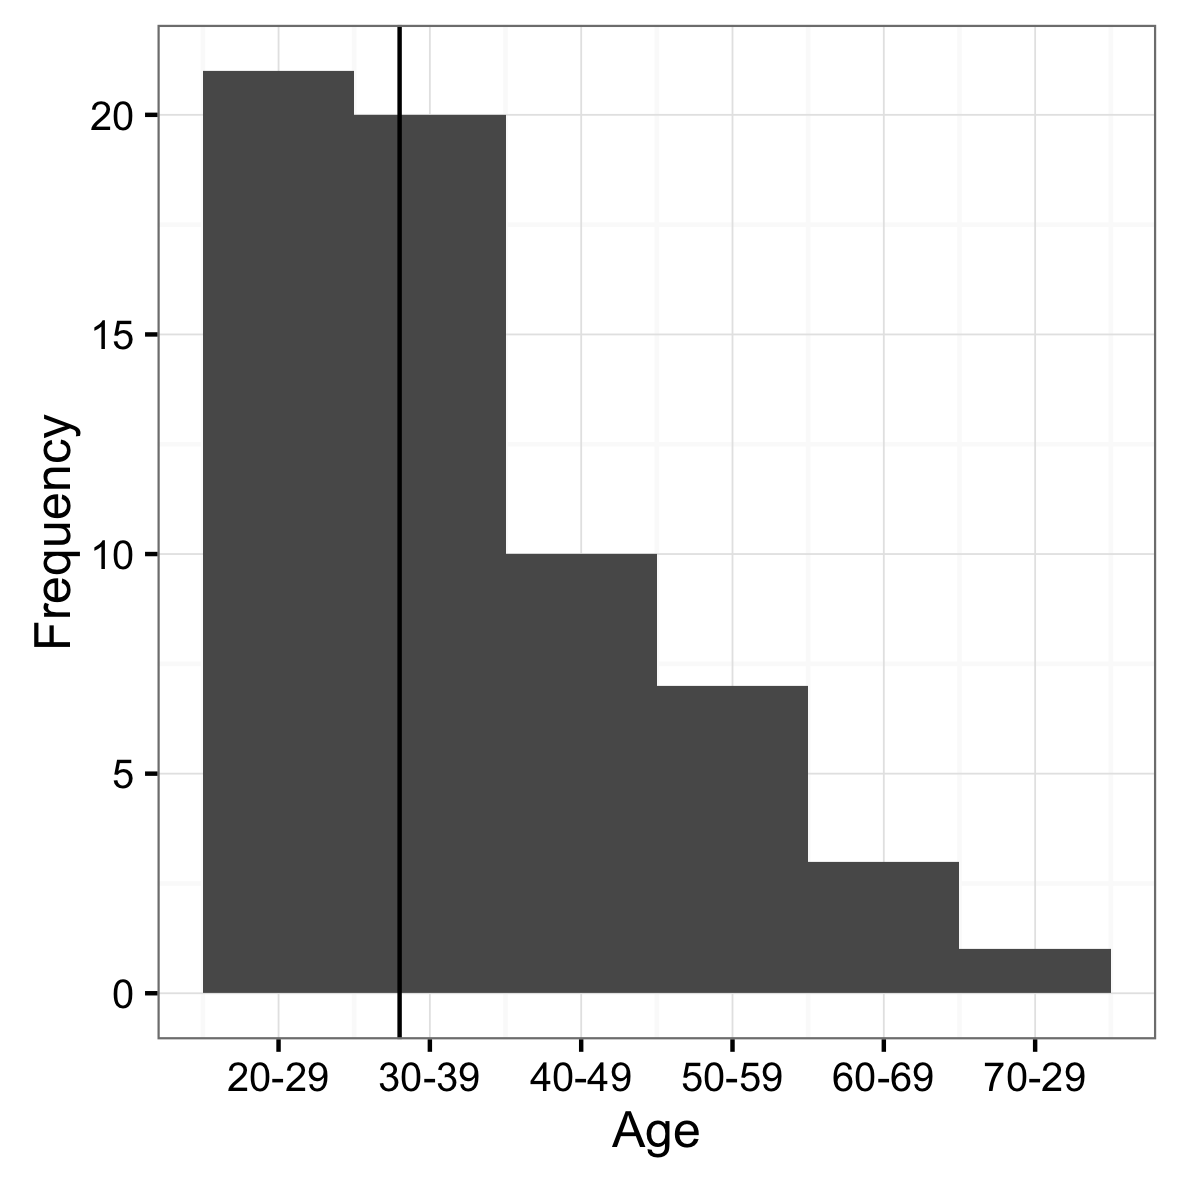
\includegraphics[width=.9\linewidth]{figures/sample2_age.png}
\caption{Distribution of age plus median in the sample of experiment 2.}
\label{fig:sample2_age}
\end{minipage}
\begin{minipage}[t]{.5\textwidth}
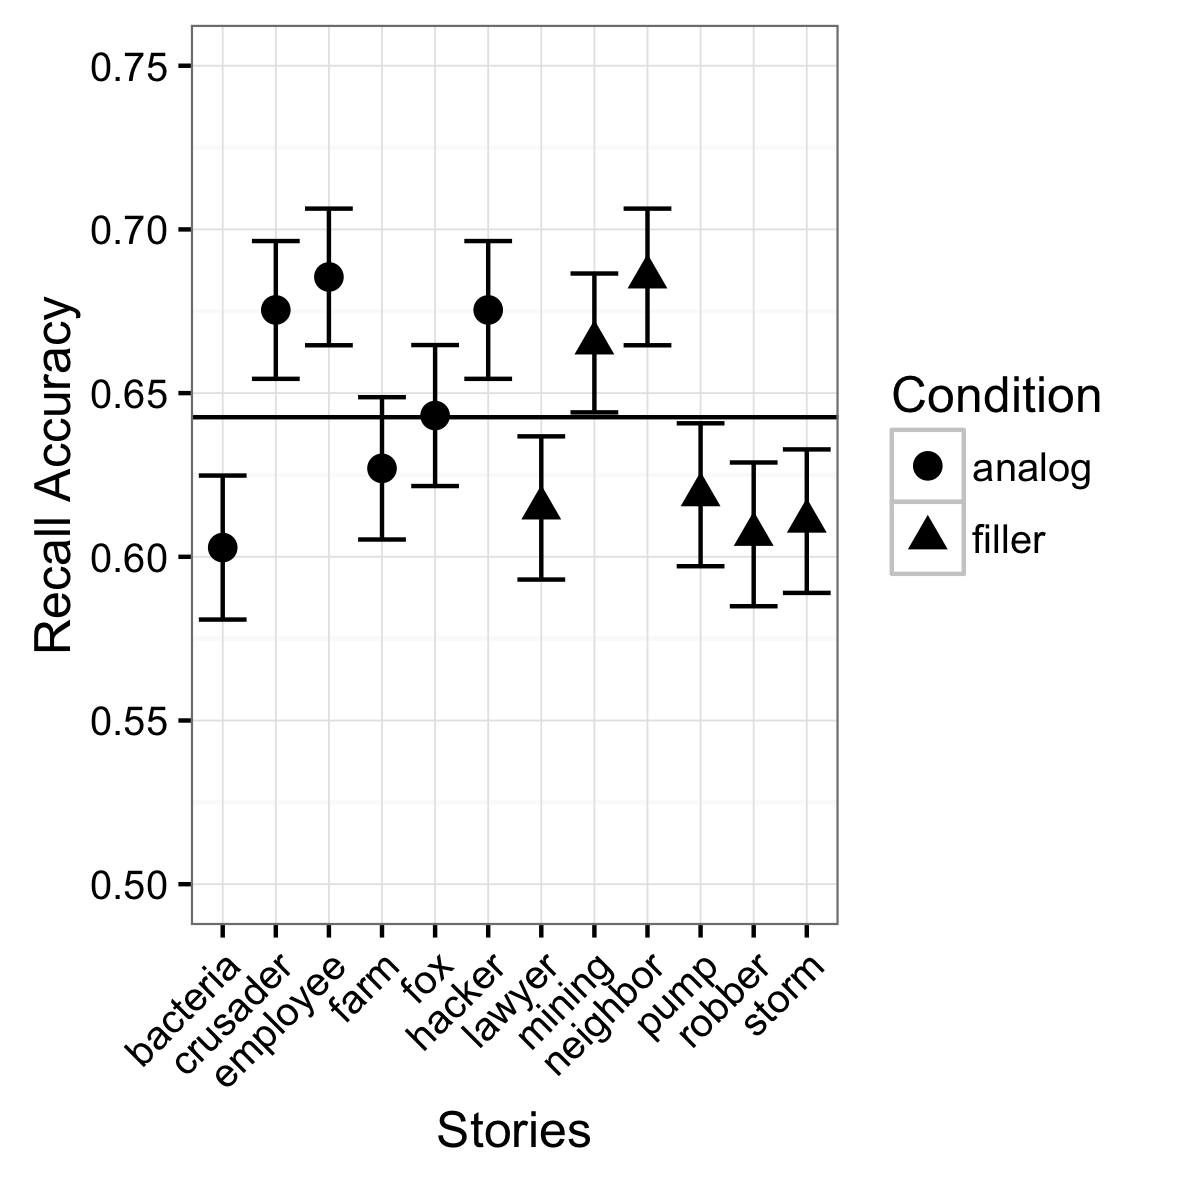
\includegraphics[width=.9\linewidth]{figures/material2_stories.png}
\caption{Mean and standard error of recall accuracy for each story with grand mean.}
\label{fig:material2_stories}
\end{minipage}
\end{figure}

\subsection{Results and Discussion}
We will only present and discuss results where they deviate from experiment 1.

\subsubsection{Material Assessment}
Even though we tried to assimilate the difficulties between the stories, it seems the reduced encoding time has introduced more sensitivity regarding story difficulty to the task (see figure \ref{fig:material2_stories}). The standard deviation between the stories mean recall accuracies are bigger in experiment 2 than in experiment 1. Although the Levene test for homogeneity of variances is just marginally significant (\textit{F}(1,24) = 3.082, \textit{p} = 0.091). Therefore the analysis of variance is again significant. But because we have less statistical power because we have less observations, this time the significance is on a lower level ( \textit{F}(11,5940) = 2.318, \textit{p} = 0.008).

\subsubsection{General Task Performance}
Setting a time limit during encoding clearly had a big impact on recall accuracy. Figure \ref{fig:genper_overall} depicts the distribution of participants' overall recall accuracy. Median is at 67\% recall accuracy, more than 10\% lower than in experiment 1. A Welch two sample t-test between subjects' overall recall accuracies from experiment 1 and 2 showed high significance (\textit{t}(147)=4.74, \textit{p} < 0.001). As a result from the increased difficulty, also the sensitivity to an individual's performance increased. The Levene test for homogeneity of variances showed a significant result (\textit{F}(1,145) = 4.0749, \textit{p} = 0.045).

\begin{figure}
\begin{minipage}[t]{.5\textwidth}
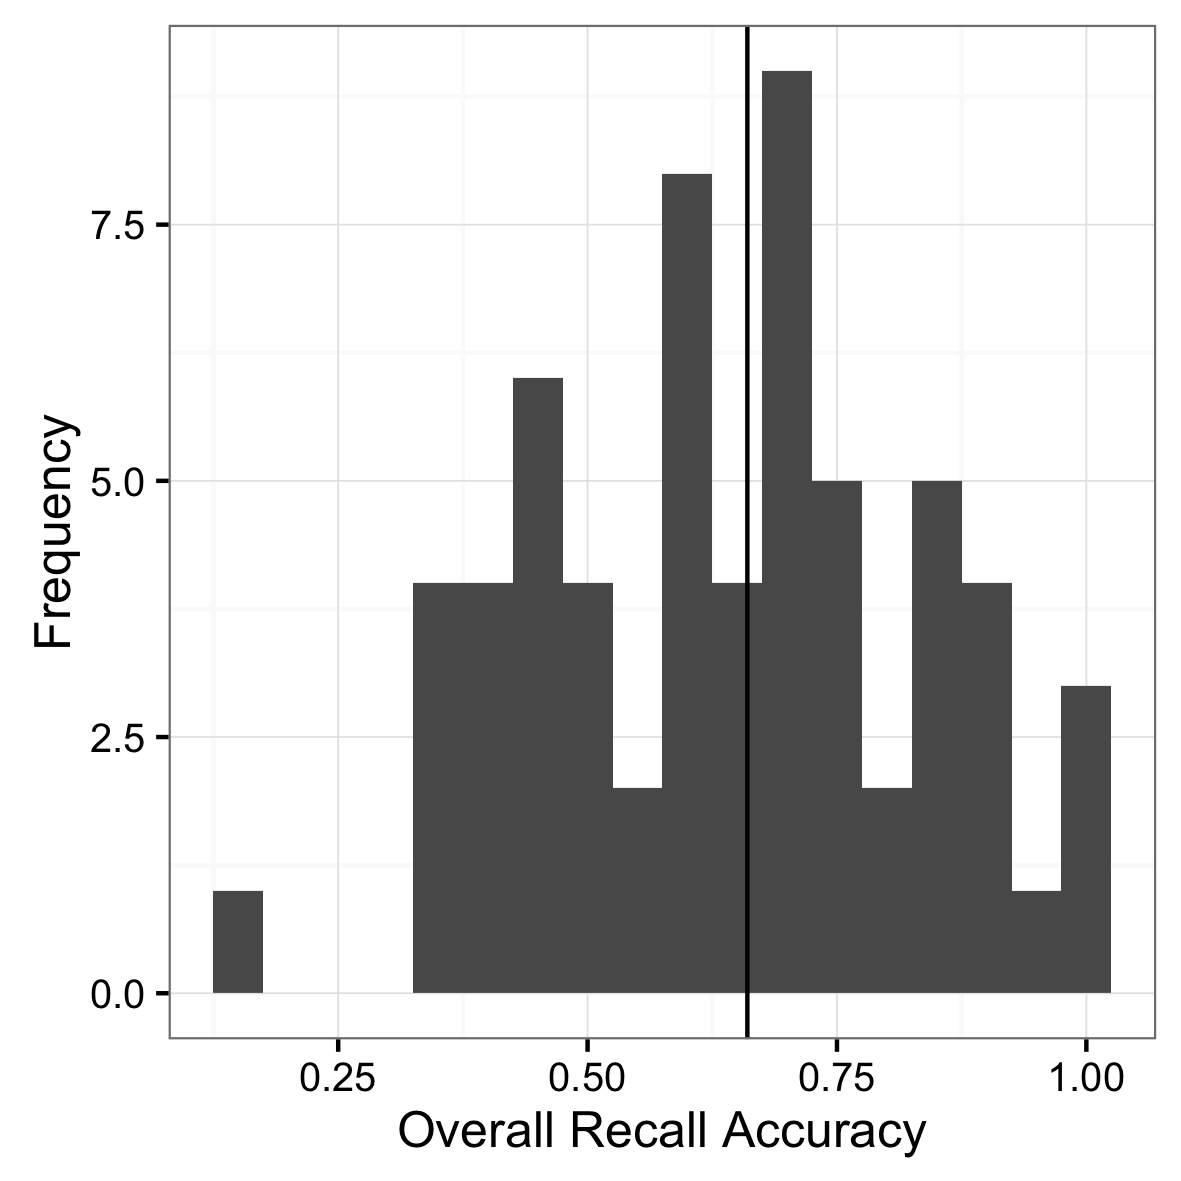
\includegraphics[width=.9\linewidth]{figures/genper2_overall.png}
\caption{Distribution of subjects' overall recall accuracy with median.}
\label{fig:genper_overall}
\end{minipage}
\begin{minipage}[t]{.5\textwidth}
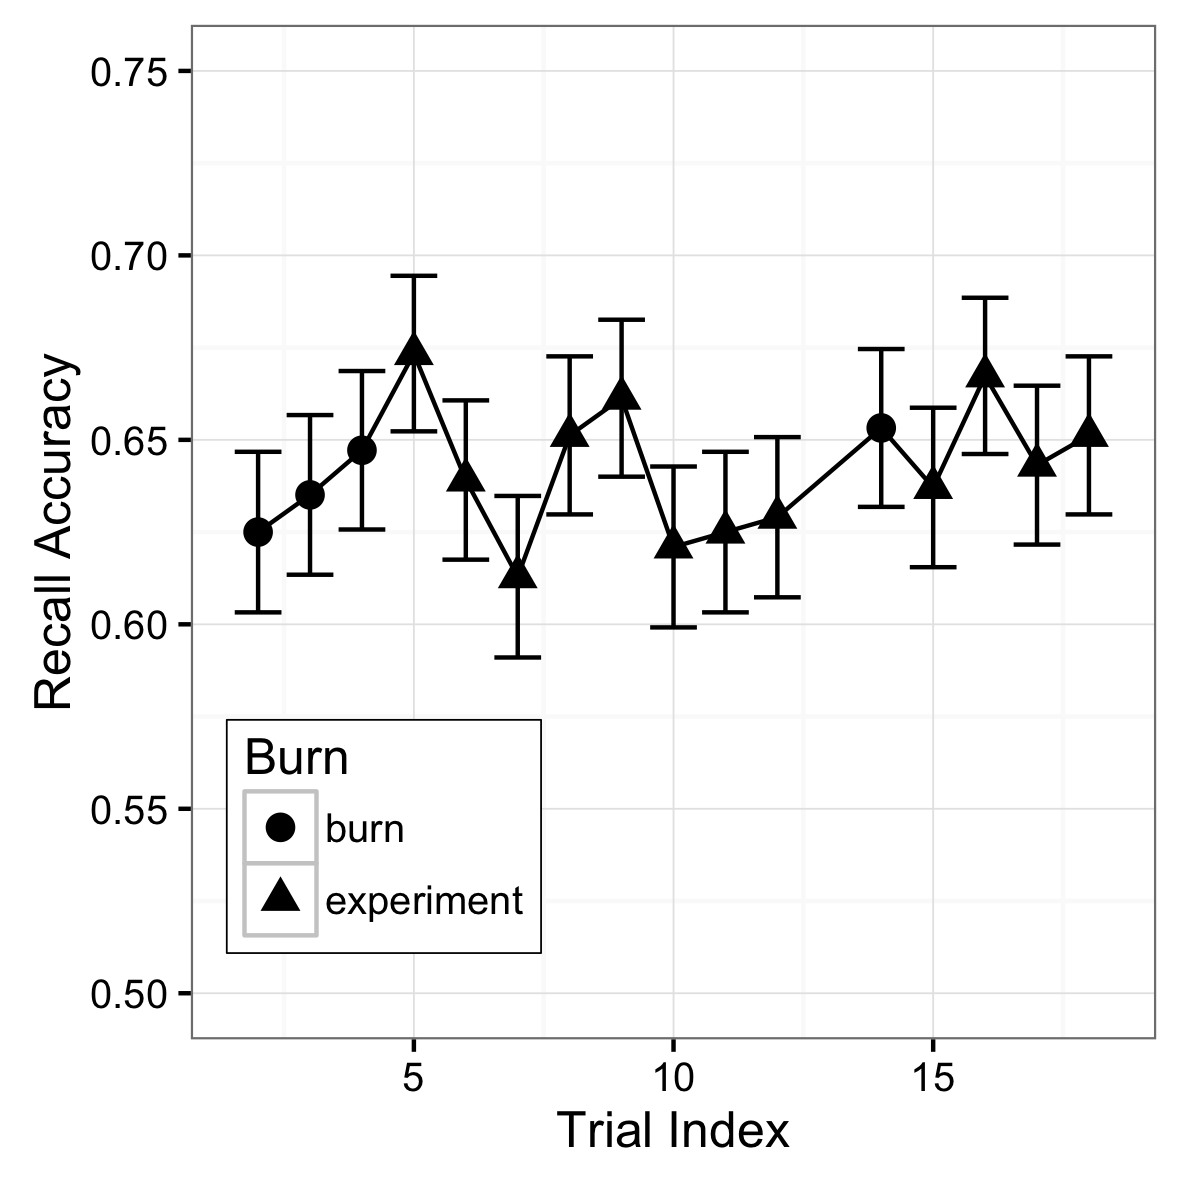
\includegraphics[width=.9\linewidth]{figures/conf2_stoIdxWburn.png}
\caption{Mean and standard error of each trial position with grand mean.}
\label{fig:conf2_stoIdx}
\end{minipage}
\end{figure}

\subsubsection{Confounding Effects}
In contrast to experiment 1 and to our surprise, we could not observe a increased memory performance effect over trial index in a simple logistic regression (\textit{e}=0.001, \textit{z}(5950)=0.194, \textit{p}=0.846). Figure \ref{fig:conf2_stoIdx} shows the absence of any tendency in recall accuracy over trial index. We can think of four reasons, why we could not replicate this finding from experiment 1.
First (a), there is no such effect in this experimental setting and the evidence in experiment 1 was obtained by chance. Second (b), the increased difficulty through the limited encoding time made the task too difficult and less sensitive to such a subtle effect. Third (c), the introduced burn phase, the first three trials in the beginning of this second experiment, took the wind out of the sails, meaning there is only an increase in recall performance over the very first few trials. And fourth (d), the samples differed regarding age which could be responsible for the absence, as age and memory performance are known to be related \citep{Hasher1988}.

The last hypothesis (d) is not supported by evidence. Even though a Welch's t-test between both sample's age distribution shows marginal significance (\textit{t}(147) = 1.81, \textit{p} = 0.073), when trying to predict subjects' overall recall accuracy with age while controlling for experiment differences, the predictor age does not play a significant role in this linear regression (\textit{e} < 0.001, \textit{t}(144) = 0.182, \textit{p} = 0.856).

The third hypothesis (c) is opposed by the fact, that even when excluding the first three trials in experiment 1, there's still a strong trial index effect on recall success in a logistic regression analysis (\textit{e} = 0.029, z(9518) = 3.558, \textit{p} < 0.001), meaning that at least in experiment 1 the first three trials are not responsible for the trial index effect. Plus, this hypothesis is also contradictory to the logistic regression including the data from burn trials in experiment 2, which also does not show a trial position effect (\textit{e} = 0.003, z(7936) = 0.626, \textit{p} = 0.532), which is also shown by figure \ref{fig:conf2_stoIdx}.

The second hypothesis (b), that the increased difficulty is responsible for a reduced sensitivity for a trial index effect, is supported by the finding that we neither detected an "after trick" and nor a "first" effect in experiment 2. In experiment 1 we observed a remarkable decrease in recall success after the trick story and greatly increased recall performance at the first trial. The logistic regression when controlling for trial index effects, neither shows significance for after trick trials (\textit{e}=0.041, \textit{z}(7936) = 0.413, \textit{p} = 0.68), nor the first trials (\textit{e} = -0.065, \textit{z}(7936) = -0.624, \textit{p} = 0.533). The concurrent absence of both effects indicate a reduced sensitivity of this experimental setting to learning effects, due to increased task difficulty.

Hypothesis one (a), that the results from experiment 1 were mere coincidence, can not be completely neglected, but given the alternative explanation for the absence of a trial index effect make it seem unlikely.

\begin{figure}
\begin{minipage}[t]{.5\textwidth}
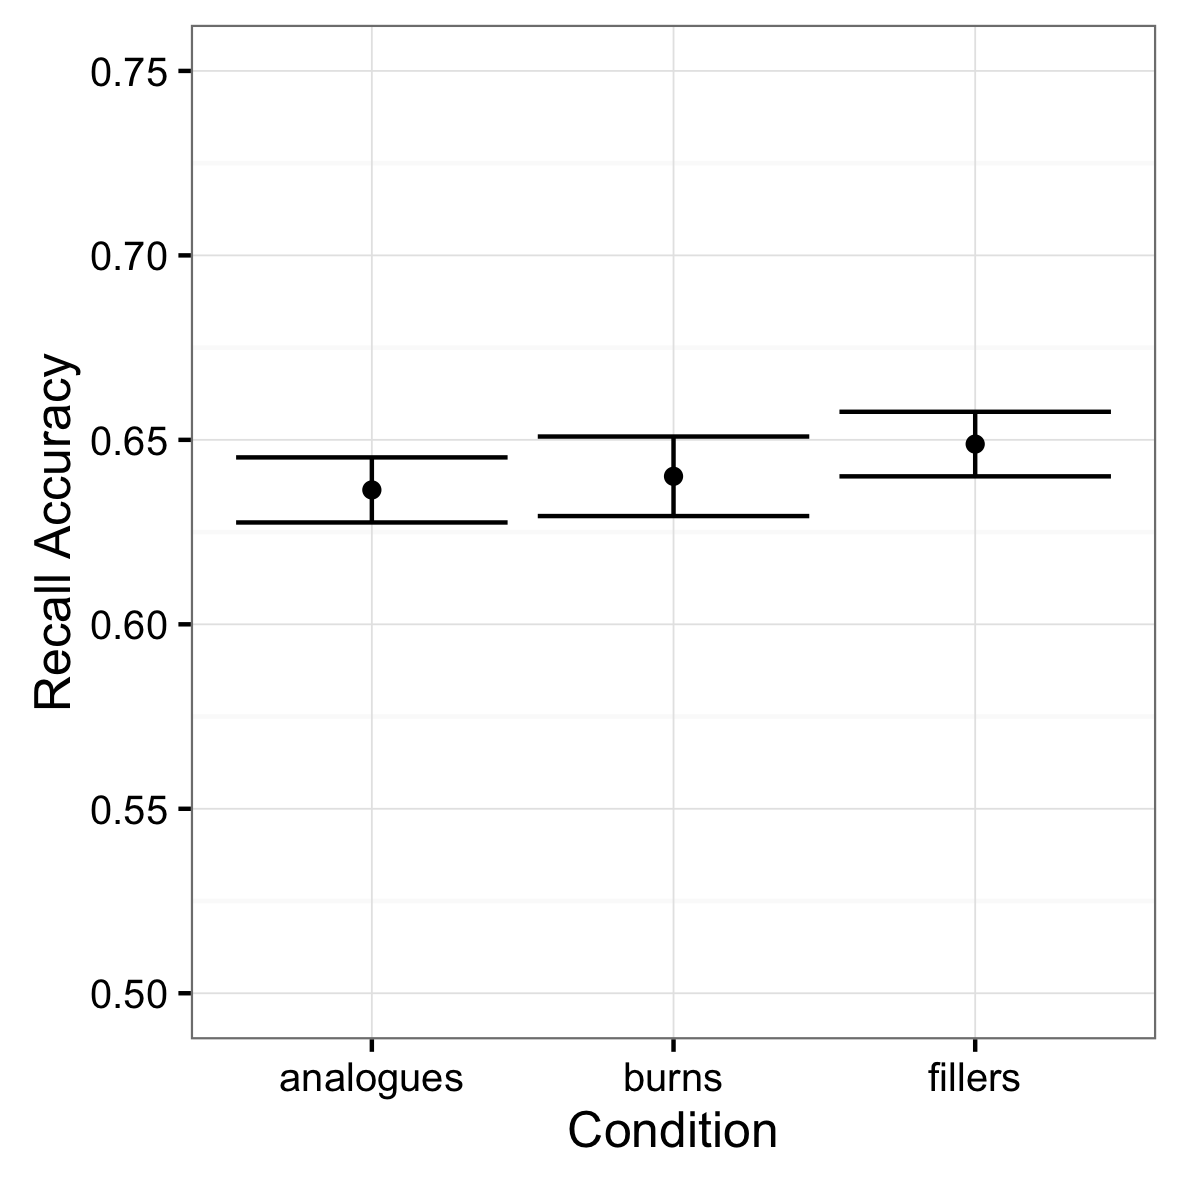
\includegraphics[width=.9\linewidth]{figures/conf2_conditionWburn.png}
\caption{Mean and standard error for each condition.}
\label{fig:conf2_conditionWburn}
\end{minipage}
\begin{minipage}[t]{.5\textwidth}
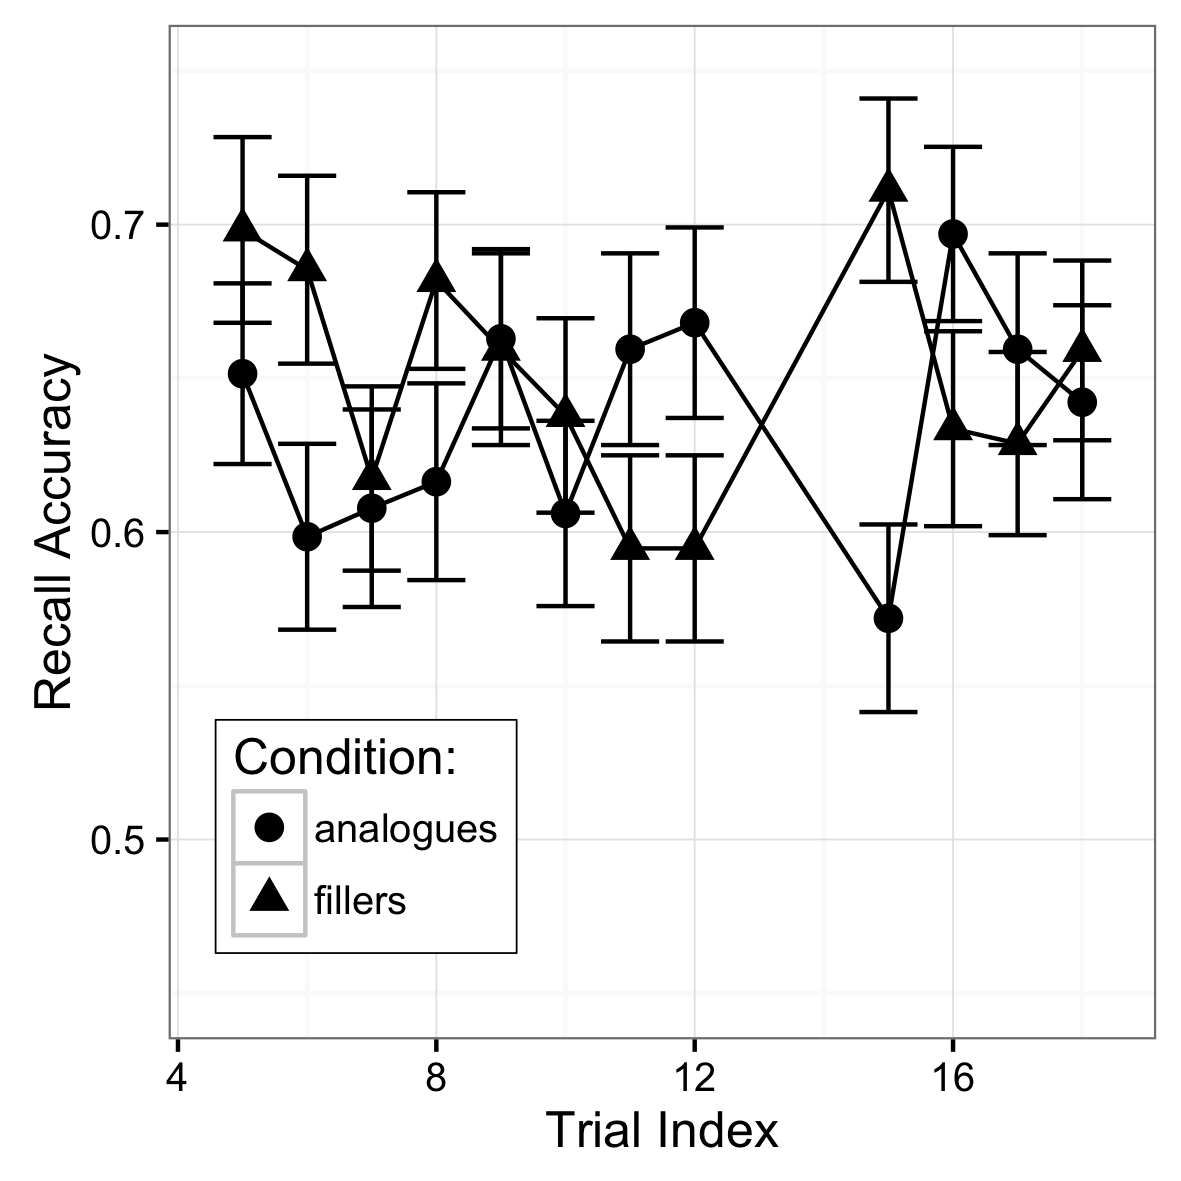
\includegraphics[width=.9\linewidth]{figures/main2.png}
\caption{Mean and standard error for each trial index and condition .}
\label{fig:main2}
\end{minipage}
\end{figure}


The other confounding effects like statement positino and response type look very much like in experiment 1, although sometimes a little different accentuated.

\subsubsection{Main Effects}


% Table created by stargazer v.5.2 by Marek Hlavac, Harvard University. E-mail: hlavac at fas.harvard.edu
% Date and time: Fri, Aug 12, 2016 - 20:03:47
\begin{table}[!htbp] \centering
  \caption{}
  \label{table:main2}
  \small
  \renewcommand{\arraystretch}{0.6}
\begin{tabular}{@{\extracolsep{5pt}}lcccc}
\\[-1.8ex]\hline
\hline \\[-1.8ex]
 & \multicolumn{4}{c}{\textit{Dependent variable:}} \\
\cline{2-5}
\\[-1.8ex] & \multicolumn{4}{c}{Recall Sucess} \\
\\[-1.8ex] & (1) & (2) & (3) & (4)\\
\hline \\[-1.8ex]
 Trial Index & 0.009 & 0.008 & 0.008 & 0.008 \\
  & (0.030) & (0.031) & (0.030) & (0.031) \\
  & & & & \\
 Response Type Relation & $-$0.496$^{**}$ & $-$0.496$^{**}$ & $-$0.497$^{**}$ & $-$0.497$^{**}$ \\
  & (0.063) & (0.063) & (0.063) & (0.063) \\
  & & & & \\
 Statement Nr 2 & $-$0.323$^{**}$ & $-$0.323$^{**}$ & $-$0.323$^{**}$ & $-$0.323$^{**}$ \\
  & (0.085) & (0.083) & (0.084) & (0.084) \\
  & & & & \\
 Statement Nr 3 & 0.692$^{**}$ & 0.692$^{**}$ & 0.693$^{**}$ & 0.693$^{**}$ \\
  & (0.096) & (0.095) & (0.096) & (0.096) \\
  & & & & \\
 Primed &  & $-$0.003 &  & $-$0.003 \\
  &  & (0.061) &  & (0.061) \\
  & & & & \\
 Condition &  & 0.026 & 0.033 & 0.030 \\
  &  & (0.047) & (0.036) & (0.048) \\
  & & & & \\
 Primed:Condition &  & 0.013 &  &  \\
  &  & (0.061) &  &  \\
  & & & & \\
 Trial Index:Condition &  &  & $-$0.035 & $-$0.034 \\
  &  &  & (0.031) & (0.031) \\
  & & & & \\
 Condition:Primed &  &  &  & 0.005 \\
  &  &  &  & (0.061) \\
  & & & & \\
 Constant & 0.941$^{**}$ & 0.943$^{**}$ & 0.942$^{**}$ & 0.944$^{**}$ \\
  & (0.167) & (0.170) & (0.167) & (0.170) \\
  & & & & \\
\hline \\[-1.8ex]
Observations & 5,952 & 5,952 & 5,952 & 5,952 \\
Log Likelihood & $-$3,321.002 & $-$3,320.571 & $-$3,319.984 & $-$3,319.979 \\
Akaike Inf. Crit. & 6,656.004 & 6,661.143 & 6,657.968 & 6,661.958 \\
Bayesian Inf. Crit. & 6,702.844 & 6,728.058 & 6,718.191 & 6,735.564 \\
\hline
\hline \\[-1.8ex]
\textit{Note:}  & \multicolumn{4}{r}{\textsuperscript{o} p<0.1; * p<0.05; ** p<0.01; *** p<0.001} \\
\end{tabular}
\end{table}


Even though we can't observe a trial index effect, there still could be an interaction with the story structure condition. An improved recall performance in the analog condition could for example be shaded by stable performance throughout the experiment in the filler condition, which could have resulted in not finding a trial index effect. Also, with the immediate repetition of the conditions, we introduced a binary variable we called "primed" in experiment 2, reflecting if the previous trial was from the same condition or not. "Primed" could show additional benefits in recall through immediate repetition of a story structure, similar to priming studies. Because we expect this effect only to appear in the analog condition, we have to test the interaction while controlling for story index effects.

Table \ref{table:main2} shows an overview of calculated logistic crossed random effects models. Figure \ref{fig:main2} shows the recall accuracy for each trial index and condition, which shows no clear tendency of an interaction between condition and trial index. This is confirmed in the model 3 and 4 of table \ref{table:main2} where the interaction shows no significance. The primed effect shows no significance in the models 2 and 4 of the same table, which can also be seen in figure \ref{fig:main2b}. The standard errors are overlapping a lot.

\begin{figure}
\begin{minipage}[t]{.5\textwidth}
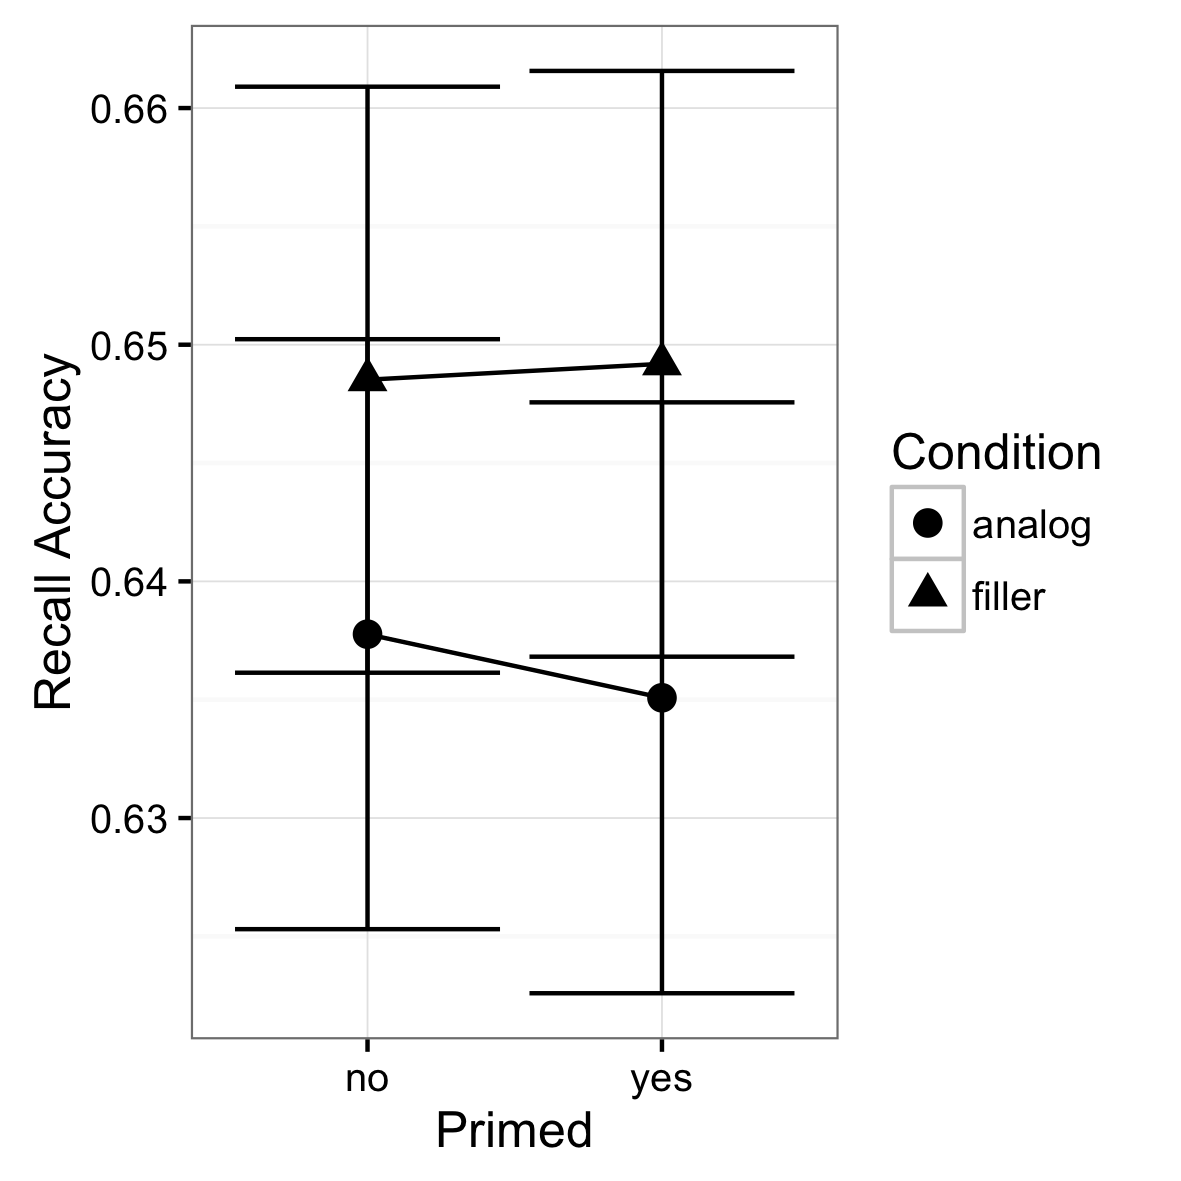
\includegraphics[width=.9\linewidth]{figures/main2b.png}
\caption{Mean and standard error for primed and condition.}
\label{fig:main2b}
\end{minipage}
\begin{minipage}[t]{.5\textwidth}
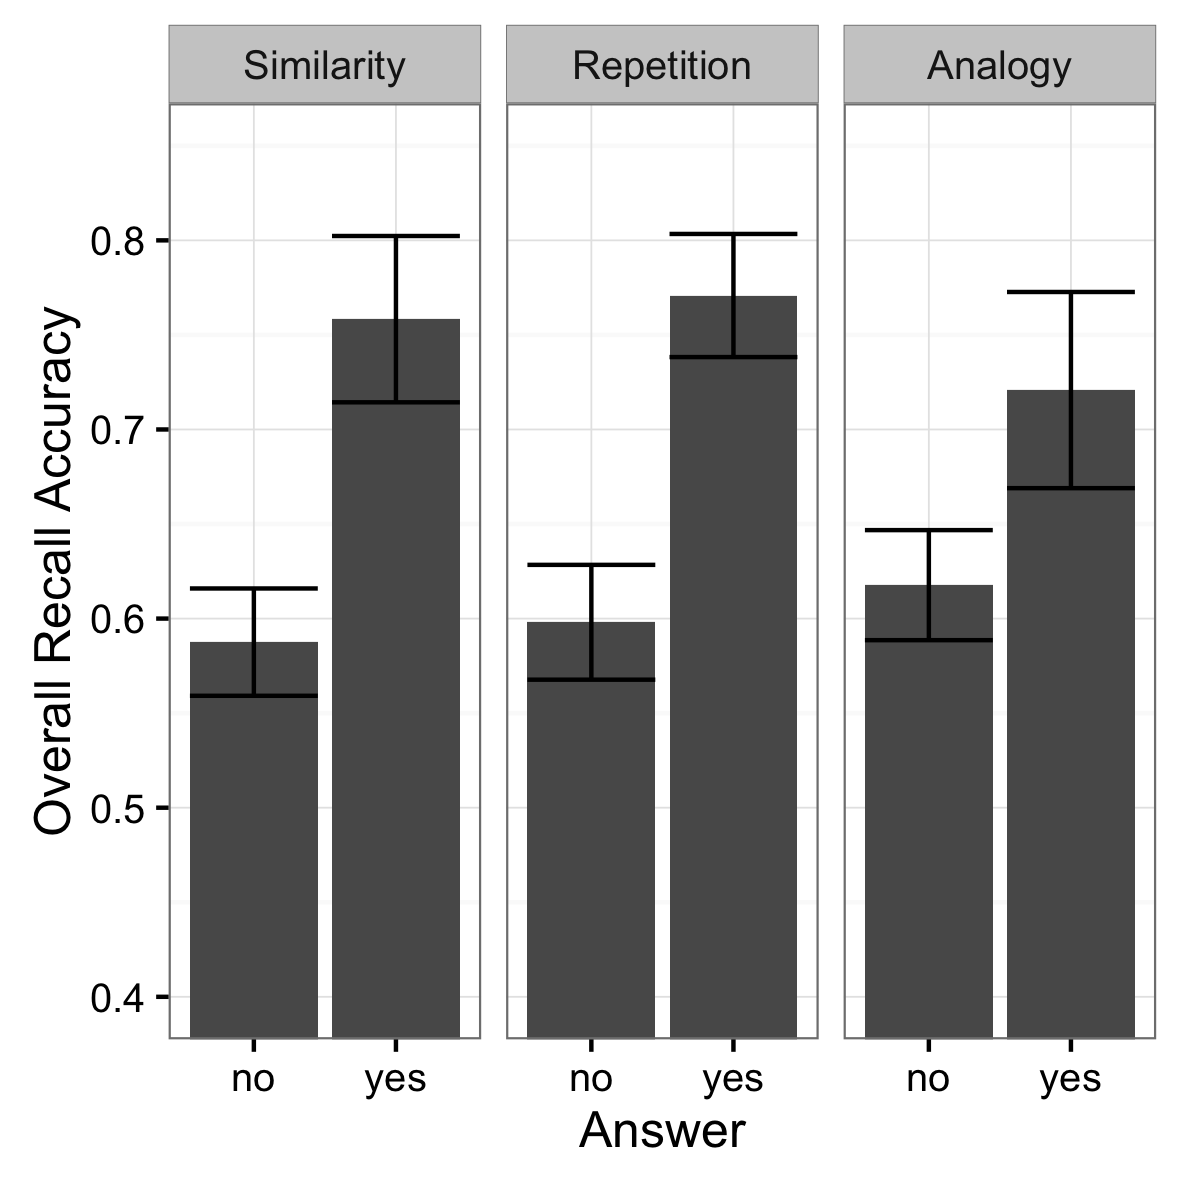
\includegraphics[width=.9\linewidth]{figures/fol2_answerXoverall.png}
\caption{Mean and standard error of subjects' recall accuracy for each follow-up question.}
\label{fig:fol2}
\end{minipage}
\end{figure}

We have already argued, that the increased task difficulty in the second experiment led to a decreased sensitivity for the trial index effect. The same could be true for even weaker effects like the interaction with condition or the effect of primed and condition. Although in this case, we have less evidence that speaks for this explanation. The alternative explanation, that those interaction effects were obtained by chance in the first experiment seems more likely, than when arguing against chance for the trial index effect.


% Table created by stargazer v.5.2 by Marek Hlavac, Harvard University. E-mail: hlavac at fas.harvard.edu
% Date and time: Fri, Aug 12, 2016 - 20:57:15
\begin{table}[!htbp] \centering
  \caption{Regression Coefficients and Standard Errors in Parentheses}
  \label{table:fol2}
  \small
  \renewcommand{\arraystretch}{0.6}
\begin{tabular}{@{\extracolsep{5pt}}lccc}
\\[-1.8ex]\hline
\hline \\[-1.8ex]
 & \multicolumn{3}{c}{\textit{Linear Regression Models predicting Overall Recall Accuracy:}} \\
\cline{2-4}
\\[-1.8ex] & (1) & (2) & (3)\\
\hline \\[-1.8ex]
 Similarity & 0.171$^{**}$ &  &  \\
  & (0.051) &  &  \\
  & & & \\
 Repetition &  & 0.173$^{**}$ &  \\
  &  & (0.055) &  \\
  & & & \\
 Analogy &  &  & 0.103$^{o}$ \\
  &  &  & (0.059) \\
  & & & \\
 Constant & 0.588$^{**}$ & 0.598$^{**}$ & 0.618$^{**}$ \\
  & (0.029) & (0.028) & (0.029) \\
  & & & \\
\hline \\[-1.8ex]
Observations & 62 & 62 & 62 \\
R$^{2}$ & 0.157 & 0.141 & 0.048 \\
Adjusted R$^{2}$ & 0.143 & 0.127 & 0.032 \\
Residual Std. Error (df = 60) & 0.188 & 0.190 & 0.200 \\
F Statistic (df = 1; 60) & 11.177$^{**}$ & 9.835$^{**}$ & 3.030$^{o}$ \\
\hline
\hline \\[-1.8ex]
\textit{Note:}  & \multicolumn{3}{r}{\textsuperscript{o} p<0.1; * p<0.05; ** p<0.01; *** p<0.001} \\
\end{tabular}
\end{table}


\subsubsection{Follow-Up}
The percentages of self-reported similarity detection between the stories were comparable to those of experiment 1. What differed though, was the effects of similarity detection on recall performance. Table \ref{table:fol2} shows an overview over three linear models predicting overall recall performance, one for each of the three follow-up questions (see appendix). Figure \ref{fig:fol2} shows the differences in recall performance with respect to similarity detection. It appears to be the case, that people that were aware of the certain similarities or repeating elements had higher recall accuracies than participants that reported to not have noted any differences. We can only speculate if this effect appeared due to an increase in task difficulty.

\subsubsection{Conclusion}
In the second experiment we could not replicate most findings from the first experiment. Setting a limit of 3 seconds per statement to read, which is less then half of the median participants used to read the statements in experiment 1, changed how trial index relates to recall performance and the interaction with story structure condition as well. We neither could observe the predicted interaction of primed structure stories with condition.

\newpage
\section{General Discussion and Future Directions}

\subsection{Material}
Materials were constructed specifically for this experiment and not validated before using it in the experiments, neither regarding their structural nor surface similarity. We only tested different story lengths to find a suitable amount of statements per story. The argument therefore can be made, that the analog stories did not actually share structural similarity, an assumption we made when building those stories. Also, we claim that our stories generally share no or only very few surface features. Through independent ratings by pairwise comparisons of stories, the subjective perceptions of those different kinds of similarities could at least be investigated.

\subsection{Processing Depth}
Another major concern regarding this experimental setup is: how well are participants integrating the information they were encoding? It is important to note this, because analog stories only share abstract information, a increased recall performance could only be observed, if the information is encoded on the required level of abstraction. The task they had to solve was pure recall and even though we are asking for relations between two entities, we did not check how well the information was integrated and how deep it was processed. Participants could just as well have remembered the sequence of items and not integrate the information in more abstract representations. Evidence that this might be important can be seen in a study from \cite{Spellman2001}. They only detected a relational priming effect when they asked participants to pay attention and use the relation. Also it seems to be the case when comparing various relational priming studies, that the kind of task participants had to do, moderates the relational priming effect \citep{Popov2015}. In one study participants were asked if a word pair makes sense \citep{Estes2006}, which requires a higher degree of information integration than for example in a lexical decision task. It could be said that our task resembles more a lexical decision task then a sensicality task in terms of information integration.

One possibility to investigate this problem in future experiments, could be to add the passively formulated relation as response options in the relation menu. Through this, it probably might not be possible to force deeper information integration during encoding, but at least it could be measured and therefore controlled, because people that only learn sequences of items and therefore integrate information less, will have more difficulties in responding to passively formulated relations. This could become visible in longer decoding times or lower recall success rates.

To incentivize deeper processing of the stories, one could also think of an additional task, like rating the sencicality of the conclusive statement, as was done in relational priming studies already \citep{Estes2006,Popov2015}. This could also be done while varying the sencicality of those statements between subjects or not. The bacteria story for example ("Bacteria \#1 emits enzyme \#2", "Enzyme \#2 dissolves the membrane of organ \#3.") could have two differing conclusive statements, i.e. "Organ \#3 fails." (original) and "Organ \#3 rules" (new and nonsensical). This addition would also be interesting to investigate, because the task would become more comparable to previous research in relational priming, when measuring reaction times of the sensicality judgement as was done before.

Individual differences regarding processing depth have not been accounted for in this thesis. According to the Theory of Cognition some people are generally more motivated to elaborate than others as kind of a personality trait \citep{Cacioppo1982,Cacioppo1996}. Therefore there also could be individual differences in our task regarding the abstraction of representations of the stories. Individual differences could be measured with either the original NFC-questionnaire \citep{Cacioppo1982} or abbreviated forms of the NFC by \cite{Epstein1996} like REI-questionnaires, which are part of the cognitive-experiential self-theory. Controlling for individual differences can reduce the noise further in a regression analysis and therefore strengthen the statistical power of a very subtle effect.

\subsection{Task difficulty}
As we have discussed already, we think that task difficulty moderates the effect of repeated story structure on recall success. The fact that more than one of the observed effects in experiment 1 are absent in experiment 2  speak for this hypothesis (interaction condition with trial index, first position, after trick position). To strengthen this argument a manipulation of the encoding time with for example 2, 4 and 8 seconds encoding time could collect further evidence in favor of this hypothesis. Also a manipulation of story length to vary task difficulty could be considered.

\newpage
\section{Summary}
The aim of this thesis was to investigate whether recall performance changes over repeated causal structures in analog stories, building on previous research from relational priming and analogical reminding studies. By combining an established method from memory research with original story material, we developed a novel experimental setting to investigate this hypothesis and contribute to growing evidence that analogical transfer happens also unintentionally. It would for the first time indicate that unintentional analogical transfer can also rely on mere structural similarity. We detected evidence for this effect in experiment 1, where we observed an interaction of story structure condition (analog vs. filler) and trial index on the the 5\%-significance level. This effect could not be replicated in experiment 2, where we changed the trial sequence to a repeated condition setting and introduced limited reading time. Because various effects from experiment 1 concurrently could not be replicated in experiment 2, we argued that the most probable reason was the increased task difficulty through the limited encoding time. We then discussed further methodological improvements and possible future experimental endeavors.


\bibliography{_main}
\section{Appendix}
\subsection{Material Experiment 1}
\subsubsection{Instructions on CrowdFlower}
In this online experiment, participants will read a few, very short stories. After each story, participants are asked to recall the content of those stories by reconstructing its statements in the order of appearance.
It will take around 20 minutes. There will be a confirmation code handed out at the end. We'll grant you a bonus of 2\$ if we can see that you showed effort. You must be a native English speaker and use a recent version of Chrome, Safari or Firefox to take part in this experiment. Means to facilitate the task are not allowed. You can only take part, if you weren't part of the same experiment already (check here).
To start the experiment, please open the following link and carefully read the instructions.

\subsubsection{Follow-Up Questions}
\begin{enumerate}
  \item Did you notice similarities between the stories during the experiment (not now)?
  \item Did you notice repeating elements between the stories during the experiment?
  \item Did you notice any repeating analog/causal structure during the experiment?
\end{enumerate}

\subsubsection{Stories with Relation Response Options}
\begin{itemize}
\item Analog Stories:
\scriptsize
\begin{longtable}{p{.08\textwidth}p{.5\textwidth}p{.42\textwidth}}
\textbf{Title} & \textbf{Statement} &\textbf{Relation-Options}\\
Bacteria & Bacteria A emits enzyme B. & emits / expels / injects \\   & Enzyme B dissolves the membrane of organ C. & dissolves sth. of / disintegrates sth. of / disjoints sth. of \\   & Organ C fails. & fails / dies / is eliminated \\  & & \\ Crusader & Crusader group A bought weapon B. & bought / acquired / caught \\   & Weapon B breaches the fortification of town C. & breaches sth. of / breaks sth. of / passes sth. of \\   & Town C is invaded. & is invaded / is intruded / is infiltrated \\  & & \\ Hacker & Hacker A wrote computer code B. & wrote / invented / thought of \\   & Code B cracks the firewall of company C. & cracks sth. of / penetrates sth. of / catches sth. of \\   & Company C suffers a data loss. & suffers sth. / leaks sth. / tolerates sth. \\  & & \\ Lawyer & Lawyer A finds loophole B. & finds / detects / meets \\   & Loophole B bypasses contract of union C. & bypasses sth. of / overrides sth. of / bystands sth. of \\   & Union C loses a lawsuit. & loses sth. / forfeits sth. / files sth. \\  & & \\ Robber & Criminal A learns about security issue B. & learns about / finds out about / starts looking \\   & Security issue B suspends alarm system of museum C. & suspends sth. of / disrupts sth. of / inspects sth. of \\   & Museum C gets robbed. & gets robbed / endures loss / is hijacked \\  & & \\ Espionage & Country A trains spy B. & trains / instructs / creates \\   & Spy B is hired by Intelligence Agency of country C. & is hired by sth. of / is employed by sth. of / is fired by sth. of \\   & Country C has its secrets stolen. & has sth. stolen / has sth. poached / has sth. lost \\  & & \\ Fox & Fox A digs tunnel B. & digs / burrow / wants \\   & Tunnel B leads to coop of chicken C. & leads to sth. of / gets to sth. of / goes on sth. of \\   & Chicken C is devoured. & is devoured / is eaten / is missing \\  & & \\
\end{longtable}
\item \normalsize Filler Stories:
\scriptsize
\begin{longtable}{p{.08\textwidth}p{.5\textwidth}p{.42\textwidth}}
Meteo & Cloud A collects humidity over ocean B. & collects humidity over / is contained in / lies in front of \\   & Ocean B lies next to the beaches of area C. & lies next to / is located near / lies above \\   & Area C is fertile. & is fertile / is humid / is rich \\  & & \\ Fish & Fisher A cultivates sea grass B. & cultivates / grows / breeds \\   & Sea grass B is eaten by fish C. & is eaten by / is consumed by / is accepted by \\   & Fish C is captured. & is captured / is taken / is digested \\  & & \\ Farm & Farmer A bought machine B. & bought / purchased / borrowed \\   & Machine B can collect fruit of plant C. & can collect / garners / can compose \\   & Plant C are harvested automatically. & are harvested automatically / are reaped mechanically / are picked manually \\  & & \\ Mining & Mining company A has a lot of resource B. & has a lot of / is filled with / fills in for \\   & Resource B is sparse in country C. & is sparse in / is rarely found in / is sparked through \\   & Country C starts negotiating. & starts negotiating / starts brokering / starts trading \\  & & \\ Insect & Perfume A attracts insect B. & attracts / lures / smells \\   & Insect B attacks woman C. & attacks / assaults / approaches \\   & Woman C has an allergic reaction. & has an allergic reaction / reacts allergically / has a panic reaction \\  & & \\ Employee & Employee A is assigned to project B. & is assigned to / is referred to / is arranged to \\   & Project B supports agenda of manager C. & supports sth. of / emphasizes sth. of / destroys sth. of \\   & Manager C gets a promotion. & gets a promotion / gets an advancement / gets a bonus \\  & & \\ School & School girl A hits boy B. & hits / punches / touches \\   & Boy B reports to teacher C. & reports to / tells / goes to \\   & Teacher C calls parents. & calls parents / notifies parents / visits parents \\  & & \\
\end{longtable}
\end{itemize}


\subsubsection{Names}
List of randomly generated names for entities in stories. Names were generated using the free online tool dialectcreator.com:\newline
Titho / Ilres / Fozeh / Thygef / Dohod / Rove / Eshbu / Ottha / Thuha / Epnux / Evib / Potho / Ribi / Kawud / Avyth / Wehif / Uyim / Saly / Ohuy / Ezol / Eshov / Lyde / Huluw / Gena / Lenik / Upum / Hoyl / Afi / Yuxeh / Thisun / Ofes / Matmag / Vuloz / Puvi / Orok / Pishi / Thyra / Diaf / Hosen / Upno / Kewos / Hoap / Adjo / Olag / Uwit / Ebib / Rivo / Uhuy / Ihab / Vivaf / Felac / Newi / Ahow / Mabi / Owih / Rothuk / Napib / Assit / Eyem / Roze / Awiz / Zimob / Ifeh / Zidep / Wutoc / Molash / Ofpoz / Mawi / Afik / Reok / Yoges / Uvman / Vilux / Lothe / Inag / Goxos / Itbob / Mewep / Ewey / Meuf / Owmi / Upel / Eefar / Igoth / Olef / Ubug / Aid / Hadith / Enmob / Wecin / Turow / Paza / Hize / Gelyp / Idog / Vipal / Pide / Gabit / Zishu / Henu / Soav / Misug / Kesal / Dugoz / Pobat / Thusoth / Ohan / Romap / Zugew / Ena / Niem

\subsection{Material Experiment 2}
\subsubsection{Instructions on CrowdFlower}
In this online experiment, participants will be asked to read very short stories and recall its content after each story. The task is hard, don't expect to remember everything, but put in effort nonetheless. We will probe your attention. It will take around 15 to 20 minutes. There will be a confirmation code handed out at the end, but only if you pay attention to the task. You must be a native English speaker and use a recent version of Chrome, Safari or Firefox to take part in this experiment. We'll hand out a 1\$ bonus if you complete and pay attention. Also you can only take part if you weren't part of another experiment from us (check here).
To start the experiment, please open the following link and carefully read the instructions: Link

\subsubsection{Stories with Relation Response Options}
\begin{itemize}
\item Analog Stories:
\scriptsize
\begin{longtable}{p{.08\textwidth}p{.5\textwidth}p{.42\textwidth}}
\textbf{Title} & \textbf{Statement} &\textbf{Relation-Options}\\
Bacteria & Bacteria A emits enzyme B. & emits / expels / injects \\   & Enzyme B dissolves the membrane of organ C. & dissolves sth. of / disintegrates sth. of / disjoints sth. of \\   & Organ C fails. & fails / dies / is eliminated \\  & & \\ Crusader & Crusader group A buys weapon B. & buys / acquires / catches \\   & Weapon B breaches the fortification of town C. & breaches sth. of / breaks sth. of / passes sth. of \\   & Town C is invaded. & is invaded / is intruded / is infiltrated \\  & & \\ Hacker & Hacker A writes computer code B. & writes / invents / thinks of \\   & Code B cracks the firewall of company C. & cracks sth. of / penetrates sth. of / catches sth. of \\   & Company C suffers a data loss. & suffers sth. / leaks sth. / tolerates sth. \\  & & \\ Lawyer & Lawyer A finds loophole B. & finds / detects / meets \\   & Loophole B bypasses contract of union C. & bypasses sth. of / overrides sth. of / bystands sth. of \\   & Union C loses a lawsuit. & loses sth. / forfeits sth. / files sth. \\  & & \\ Robber & Criminal A learns about security issue B. & learns about / finds out about / starts looking \\   & Security issue B suspends alarm system of museum C. & suspends sth. of / disrupts sth. of / inspects sth. of \\   & Museum C gets robbed. & gets robbed / endures loss / is hijacked \\  & & \\ Fox & Fox A digs tunnel B. & digs / burrow / wants \\   & Tunnel B leads to coop of chicken C. & leads to sth. of / gets to sth. of / goes on sth. of \\   & Chicken C is devoured. & is devoured / is eaten / is missing \\  & & \\
\end{longtable}
\item \normalsize Filler Stories:
\scriptsize
\begin{longtable}{p{.08\textwidth}p{.5\textwidth}p{.42\textwidth}}
Storm & Storm A hits tree B. & hits / blows off / runs over \\   & Tree B falls on trail of route C. & falls on / drops on / is thrown on \\   & Route C is blocked. & is blocked / is jammed / is ruined \\  & & \\ Farm & Farmer A purchases machine B. & purchases / buys / borrows \\   & Machine B can collect fruit of plant C. & can collect / garners / can compose \\   & Plant C are harvested automatically. & are harvested automatically / are reaped mechanically / are picked manually \\  & & \\ Mining & Mining company A has a lot of resource B. & has a lot of / is filled with / fills in for \\   & Resource B is sparse in country C. & is sparse in / is rarely found in / is sparked through \\   & Country C starts negotiating. & starts negotiating / starts brokering / starts trading \\  & & \\ Pump & Plumber A installs pump B. & installs / builds / fixes \\   & Pump B sucks water from ground C. & sucks sth. from / transports sth. from / elevates sth. from \\   & Ground C dries up. & dries up / dehydrates / soakes up \\  & & \\ Employee & Employee A is assigned to project B. & is assigned to / is referred to / is arranged to \\   & Project B supports agenda of manager C. & supports sth. of / emphasizes sth. of / destroys sth. of \\   & Manager C gets a promotion. & gets a promotion / gets an advancement / gets a bonus \\  & & \\ Neighbor & Man A takes care of cat B. & takes care of / looks after / is feeding \\   & Cat B walks over the flowers of neighbor C & walks over sth. of / goes over sth. of / strays over to \\   & Neighbor C gets angry. & gets angry / becomes furious / gets aroused \\  & & \\
\end{longtable}
\item \normalsize Burn-In Stories:
\scriptsize
\begin{longtable}{p{.08\textwidth}p{.5\textwidth}p{.42\textwidth}}
Fish & Fisher A cultivates sea grass B. & cultivates / grows / breeds \\   & Sea grass B is eaten by fish C. & is eaten by / is consumed by / is accepted by \\   & Fish C is captured. & is captured / is taken / is digested \\  & & \\ School & School girl A beats boy B. & beats / punches / touches \\   & Boy B reports to teacher C. & reports to / tells / goes to \\   & Teacher C calls parents. & calls parents / notifies parents / visits parents \\  & & \\ Insect & Perfume A attracts insect B. & attracts / lures / smells \\   & Insect B attacks woman C. & attacks / assaults / approaches \\   & Woman C has an allergic reaction. & has an allergic reaction / needs medical support / has a panic reaction \\  & & \\ Meteo & Cloud A collects humidity over ocean B. & collects humidity over / is contained in / lies in front of \\   & Ocean B lies next to the beaches of area C. & lies next to / is located near / lies above \\   & Area C is fertile. & is fertile / is humid / is rich \\  & & \\
\end{longtable}
\end{itemize}


\includepdf{selbstaendigkeit}
\end{document}
